\documentclass[a4paper]{article}

%use the english line for english reports
%usepackage[english]{babel}
\usepackage[portuguese]{babel}
\usepackage[utf8]{inputenc}
\usepackage{indentfirst}
\usepackage{graphicx}
\usepackage{verbatim}
\usepackage{fancyhdr}
\usepackage{listings}
\usepackage{color}

\definecolor{dkgreen}{rgb}{0,0.6,0}
\definecolor{gray}{rgb}{0.5,0.5,0.5}
\definecolor{mauve}{rgb}{0.58,0,0.82}

\lstset{frame=tb,
  language=Prolog,
  aboveskip=3mm,
  belowskip=3mm,
  showstringspaces=false,
  columns=flexible,
  basicstyle={\small\ttfamily},
  numbers=none,
  numberstyle=\tiny\color{gray},
  keywordstyle=\color{blue},
  commentstyle=\color{dkgreen},
  stringstyle=\color{mauve},
  breaklines=true,
  breakatwhitespace=true,
  tabsize=3
  }

\begin{document}


\setlength{\textwidth}{16cm}
\setlength{\textheight}{22cm}

\title{\Huge\textbf{FABRIK}\linebreak\linebreak\linebreak
\Large\textbf{Relatório Final}\linebreak\linebreak
\linebreak\linebreak

\includegraphics[scale=0.1]{images/feup-logo.png}\linebreak\linebreak
\linebreak\linebreak
\Large{Mestrado Integrado em Engenharia Informática e Computação} \linebreak\linebreak
\Large{Programação em Lógica}\linebreak
}

\author{\textbf{Grupo Fabrik3:}\\
\linebreak\\
André Cruz - 201503776 \\
Edgar Carneiro - 201503748 \\
\linebreak\linebreak \\
 \\ Faculdade de Engenharia da Universidade do Porto \\ Rua Roberto Frias, s\/n, 4200-465 Porto, Portugal \linebreak\linebreak\linebreak
\linebreak\linebreak\vspace{1cm}}

\maketitle
\thispagestyle{empty}

%************************************************************************************************
%************************************************************************************************

\newpage

\section*{Resumo}

Este trabalho tem como objetivo a modelação e implementação do jogo de tabuleiro \textit{Fabrik}, com uma representação na linha de comandos, e disponibilizando os modos de jogo \textit{jogador vs jogador}, \textit{jogador vs computador} e \textit{computador vs computador}. Tratando-se de um jogo de tabuleiro, foi necessário decidir um modelo apropriado para representar o estado do jogo, desenvolver predicados para verificar se determinada jogada é válida, e predicados para determinar quando o jogo termina. Foi também necessário implementar resilientes mecanismos de obtenção de \textit{input} do utilizador, e menus para interface com o utilizador.

Relativamente à escolha automática de uma jogada por parte do computador, esta tem dois níveis: um mais fácil, em que a jogada é escolhida aleatoriamente; e um mais difícil, em que é identificada a melhor jogada que é possível efetuar tendo em conta o contexto atual (algoritmo ganancioso). Neste sentido, desenvolvemos vários predicados para a avaliação quantitativa de uma jogada e do estado do jogo, tendo sido alcançados os nossos objetivos de dificuldade de jogo contra o computador.

Recorrendo à excelente bibliografia indicada pelos professores, \cite{sterling_shapiro_warren_2010} e \cite{carlsson_fruhwirth_2016}, foi possível resolver todos os problemas que encontramos na implementação deste jogo, bem como uma aprendizagem contínua dos conceitos relacionados com este paradigma de programação.

Para finalizar, achamos que o trabalho apresentado representa uma eficiente, completa e compreensiva modelação do jogo \textit{Fabrik} e dos seus conceitos, e temos orgulho no resultado final.

\newpage

\tableofcontents

%************************************************************************************************
%************************************************************************************************

%*************************************************************************************************
%************************************************************************************************

\newpage

%%%%%%%%%%%%%%%%%%%%%%%%%%
\section{Introdução}

Este trabalho foi desenvolvido no âmbito da unidade curricular de Programação em Lógica, integrada no 3º ano do Mestrado Integrado em Engenharia Informática e Computação, tendo como objetivo aprofundar os conhecimentos adquiridos nas aulas teóricas e práticas desta unidade curricular, bem como a abordagem de problemas mais práticos com recurso à linguagem \textit{PROLOG}. Deste modo, propusemo-nos a implementar e modelar do jogo de tabuleiro \textit{Fabrik}, sendo possível os modos de jogo \textit{jogador vs jogador}, \textit{jogador vs computador} e \textit{computador vs computador} (com dois níveis de dificuldade).

A escolha deste jogo, que foi selecionado dentro de um leque de opções disponibilizadas pelos docentes, prendeu-se no conjunto de conceitos intuitivos que incorpora (\textit{e.g.} linhas de visão das peças), permitindo uma rápida aprendizagem das regras, assim como um desafio na implementação de restrições de jogadas e avaliação do tabuleiro. Esta aparente simplicidade é no entanto contrabalançada com o facto de cada jogada ter dois passos: a colocação do \textit{worker}, e a colocação de uma peça \textit{black}/\textit{white} (estando este segundo passo fortemente constrangido pelo primeiro).

Este relatório está dividido em várias secções, sendo a presente a primeira:
\begin{enumerate}
\item Na segunda secção deste relatório, é feita uma pequena introdução à história do jogo \textit{Fabrik}, aos componentes físicos necessários para jogar, e às regras oficiais do jogo;
\item Na secção seguinte, são apresentados vários detalhes da nossa implementação, desde a representação visual do tabuleiro ao algoritmo de cálculo da melhor jogada possível dado um determinado estado de jogo;
\item Na quarta secção, é descrita a interface com o utilizador, que consiste nos menus e input esperado em cada um destes;
\item Na última secção, são tecidas conclusões acerca do desenvolvimento deste trabalho e do seu enquadramento curricular.
\end{enumerate}

\newpage

%%%%%%%%%%%%%%%%%%%%%%%%%%
\section{O Jogo \textit{Fabrik}}

\subsection{História}
O jogo - \textit{Fabrik} - foi recentemente desenvolvido por Dieter Stein, em agosto de 2017, como parte de um estudo para o desenvolvimento de um novo jogo, Urbino.

\subsection{Material}
\begin{itemize}
	\item Tabuleiro quadrangular
	\item Quantidade suficiente de peças pretas e brancas
	\item Duas peças vermelhas chamadas trabalhadores
\end{itemize}

\begin{figure}[h!]
\begin{center}
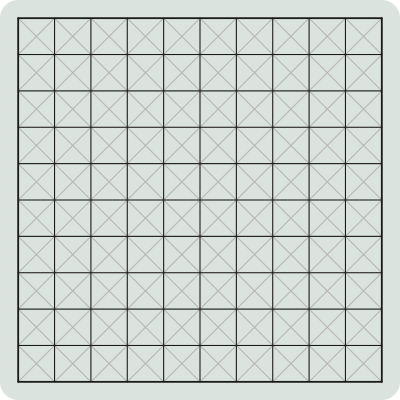
\includegraphics[height=3cm,width=3cm]{images/fabrik_empty_board.png}
\caption{Tabuleiro vazio de 11 x 11 espaços}
\label{Figura 1}
\end{center}
\end{figure}

\subsection{Regras}
A implementação deste jogo foi baseada no manual de regras oficiais \cite{games_and_puzzles_by_dieter_stein}.

As pretas (jogador que joga com peças de cor preta) começam por colocar um dos trabalhadores num espaço à sua escolha. De seguida, as brancas (jogador que joga com peças de cor branca) colocam o outro trabalhador num espaço livre. De seguida, as pretas decidem quem começa por jogar.

O jogo procede por turnos, sendo que em cada turno um jogador pode, se assim optar, mover um dos trabalhadores para um espaço vazio. De seguida, o jogador deve jogar colocar uma das suas peças num ponto de interseção entre as “linhas de visão dos dois trabalhadores”. As linhas de visão dos trabalhadores são as linhas na diagonal, horizontal e vertical sobre as quais os trabalhadores se encontram posicionados.

\begin{figure}[h!]
\begin{center}
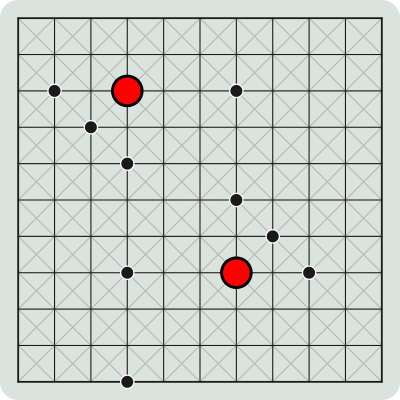
\includegraphics[height=3cm,width=3cm]{images/fabrik_intersection.png}
\caption{Pontos de interseção entre os dois trabalhadores}
\label{Figura 2}
\end{center}
\end{figure}

No caso especial em que os dois trabalhadores se encontram sobre uma mesma linha ortogonal ou diagonal, apenas os espaços entre eles são considerados pontos de interseção (se estiverem vazios), ao invés da totalidade dessa linha.

Ganha o jogo o jogador que consiga criar uma linha de pelo menos 5 pedras da sua cor, ortogonal ou diagonalmente. Um jogador ganha também o jogo se o seu adversário não conseguir posicionar nenhum dos trabalhadores de forma a poder colocar uma pedra sua no tabuleiro.

\begin{figure}[h!]
\begin{center}
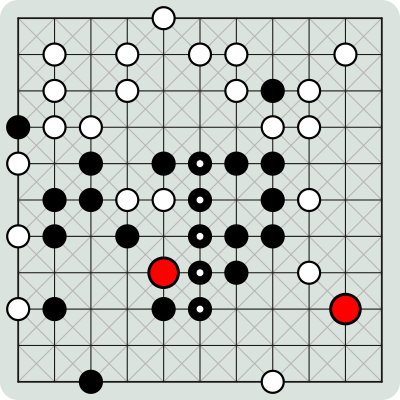
\includegraphics[height=3cm,width=3cm]{images/fabrik_full_board.png}
\caption{Final de uma partida de Fabrik, com vitórias das pretas}
\label{Figura 3}
\end{center}
\end{figure}


\newpage

%%%%%%%%%%%%%%%%%%%%%%%%%%
\section{Lógica do Jogo}

Descrever o projeto e implementação da lógica do jogo em Prolog, incluindo a forma de representação do estado do tabuleiro e sua visualização, execução de movimentos, verificação do cumprimento das regras do jogo, determinação do final do jogo e cálculo das jogadas a realizar pelo computador utilizando diversos níveis de jogo. Sugere-se a estruturação desta secção da seguinte forma:

\subsection{Representação do Estado do Jogo}

A representação dos estados de jogo é feita com recurso a uma lista de listas, de forma a simular o uso de uma Matriz. Seguem de seguida a representação de diferentes estados de jogo:\newline


Representação do \textbf{estado inicial}:

\begin{small}
\begin{lstlisting}
[[none, none, none, none,  none, none,  none, none, none, none, none],
 [none, none, none, none,  none, none,  none, none, none, none, none],
 [none, none, none, none,  none, none,  none, none, none, none, none],
 [none, none, none, none,  none, none,  none, none, none, none, none],
 [none, none, none, none,  none, none,  none, none, none, none, none],
 [none, none, none, none,  none, none,  none, none, none, none, none],
 [none, none, none, none,  none, none,  none, none, none, none, none],
 [none, none, none, none,  none, none,  none, none, none, none, none],
 [none, none, none, none,  none, none,  none, none, none, none, none],
 [none, none, none, none,  none, none,  none, none, none, none, none],
 [none, none, none, none,  none, none,  none, none, none, none, none]]
\end{lstlisting}
\end{small}

\begin{figure}[h!]
\centering
\begin{minipage}{.35\textwidth}
	\centering
	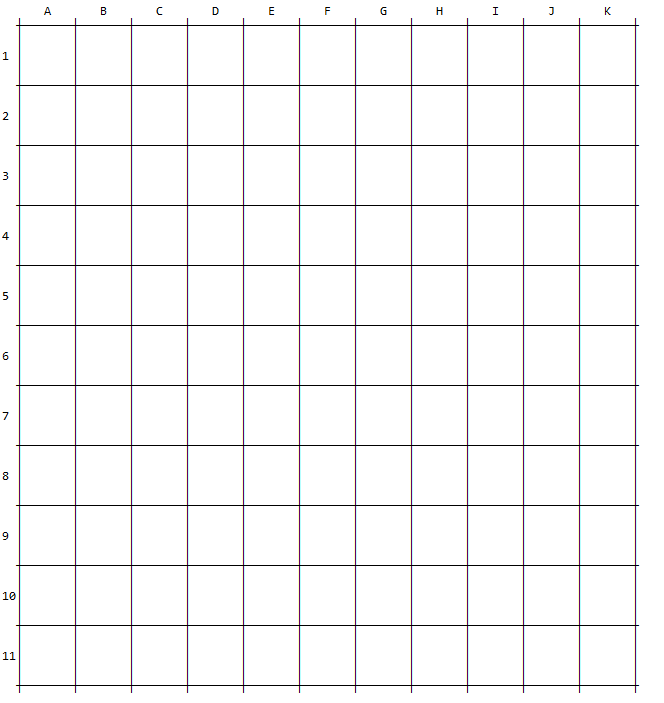
\includegraphics[width=\textwidth]{images/self_empty_board.png}
	\caption{Representação do estado inicial na consola}
	\label{Figura 4}
\end{minipage}
\quad \quad
\begin{minipage}{.35\textwidth}
	\centering
	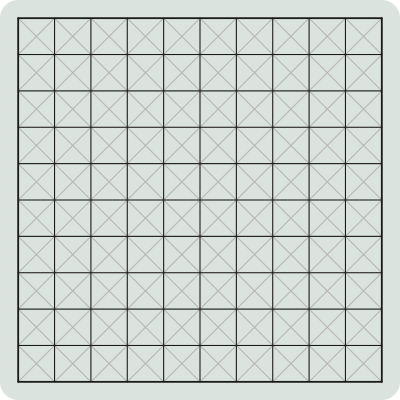
\includegraphics[width=\textwidth]{images/fabrik_empty_board.png}
	\caption{Tabuleiro original Vazio}
	\label{Figura 5}
\end{minipage}
\end{figure}

\clearpage

Representação de um possível \textbf{estado intermédio}:\newline

\begin{small}
\begin{lstlisting}
[[ none, none, none, none, none, none, none, none, none, none, none],
 [ none, none, none, none, none, white, worker, none, none, none, none],
 [ none, none, none, none, none, none, white, black, white, none, none],
 [ none, white, white, none, none, none, none, white, white, none, none],
 [white, none, none, none, black, black, none, black, none, none, none],
 [ none, none, black, white, none, none, none, none, white, none, none],
 [ none, black, none, none, none, black, black, black, none, none, none],
 [ none, none, none, none, none, none, black, none, white, none, none],
 [ none, none, none, none, none, black, none, none, none, none, none],
 [ none, none, none, none, worker, none, none, none, none, none, none],
 [ none, none, none, none, none, none, none, none, none, none, none]]
\end{lstlisting}
\end{small}

\begin{figure}[h!]
\begin{center}
	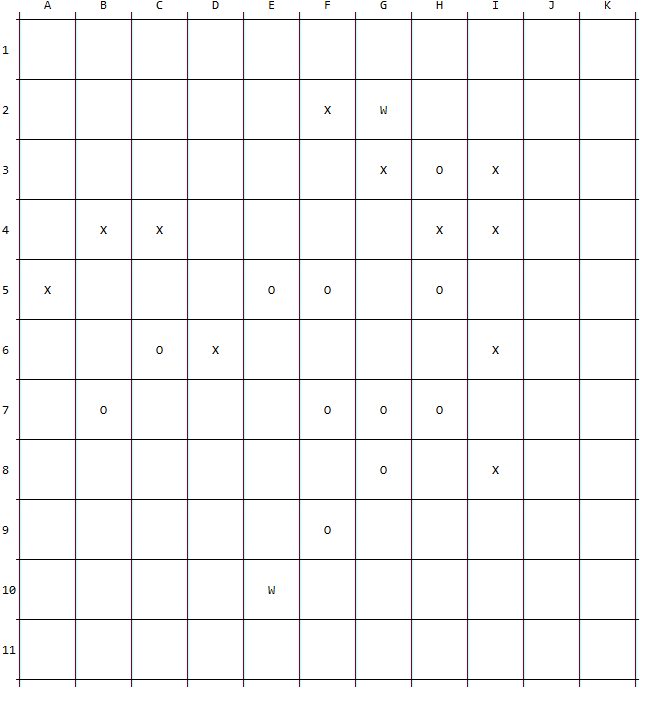
\includegraphics[height=6cm, width=6cm]{images/self_semi_board.png}
	\caption{Representação na consola, de um possível estado intermédio}
	\label{Figura 6}
\end{center}
\end{figure}

\clearpage
Representação de um possível \textbf{estado final}:\newline

\begin{small}
\begin{lstlisting}
[[ none, none, none, none, white, none, none, none, none, none, none],
 [ none, white, none, white, none, white, white, none, none,white, none],
 [ none, white, none, white, none, none,white, black, white, none, none],
 [black, white, white, none, none, none, none, white, white, none, none],
 [white, none, black, none,black, black, black, black, none, none, none],
 [none, black, black, white,white, black, none, black,white, none, none],
 [white, black, none,black, none, black, black, black, none, none, none],
 [ none, none, none, none, worker, black, black, none,white, none, none],
 [white, black, none, none,black, black, none, none, none, worker, none],
 [ none, none, none, none, none, none, none, none, none, none, none],
 [ none, none, black, none, none, none, none, white, none, none, none]]
\end{lstlisting}
\end{small}

\begin{figure}[h!]
\centering
\begin{minipage}{.35\textwidth}
	\centering
	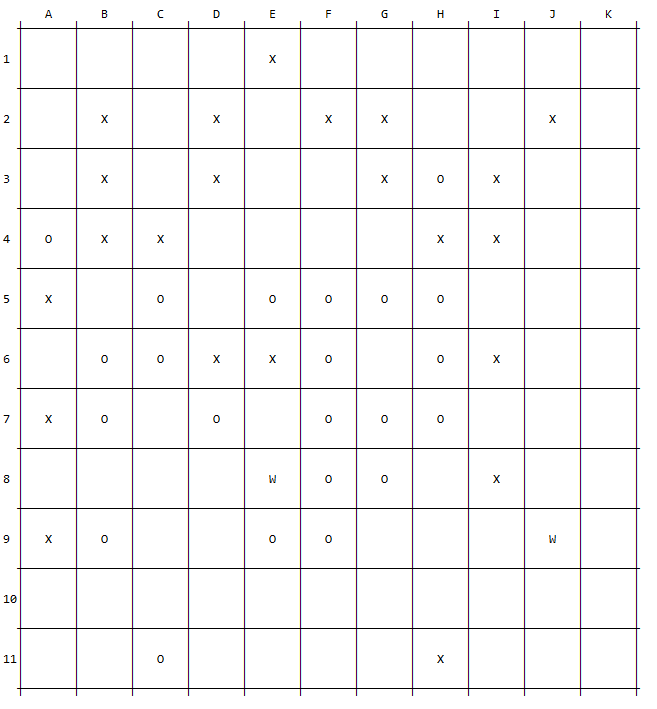
\includegraphics[width=\textwidth]{images/self_full_board.png}
	\caption{Representação do estado final na consola}
	\label{Figura 7}
\end{minipage}
\quad \quad
\begin{minipage}{.35\textwidth}
	\centering
	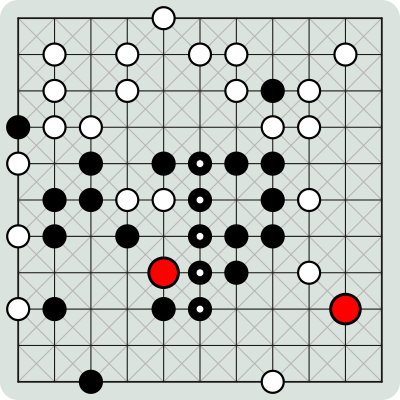
\includegraphics[width=\textwidth]{images/fabrik_full_board.png}
	\caption{Representção do mesmo estado final, no tabuleiro original}
	\label{Figura 8}
\end{minipage}
\end{figure}

\clearpage


%%%%%%%%%%%%%%%%%%%%%%%%%%
\subsection{Visualização do Tabuleiro}

Para a representação do tabuleiro em modo de texto, foi criado o seguinte código em prolog:
\begin{lstlisting}[language=prolog]
% Dictionary for Board Elements
translate(none, 32). %Empty Cell
translate(black, 79). %Dark Pieces
translate(white, 88). %White Pieces
translate(worker, 9608). %Red Workers

(...)

% General PrintBoard
printBoard(Board):-
        boardSize(N),
        printBoard(Board, N), !.

% Board Printing - arguments: Board and Board size
printBoard(Board, N):-
        clearConsole,
        write('  '), printHorizontalLabel(N, N),
        printBoard(Board, N, 1), !.

printBoard([], N, _):-
        printRowDivider(N), nl.

printBoard([Line | Board], N, CurrentL):-
        printRowDivider(N),
        printDesignRow(N),
        printVerticalLabel(CurrentL),
        put_code(9474),
        printLine(Line),
        printDesignRow(N),
        NewL is (CurrentL + 1),
        printBoard(Board, N, NewL).

printLine([]):- nl.
printLine([Head | Tail]) :-
        translate(Head, Code),
        write('   '),
        put_code(Code),
        write('   '), put_code(9474),
        printLine(Tail).

%  AESTHETICS

printRowDivider(N):-
        write('  '),
        put_code(9532),
        printRowDividerRec(N).

printRowDividerRec(0) :- nl.
printRowDividerRec(N) :-
        put_code(9472), put_code(9472), put_code(9472), put_code(9472),
        put_code(9472), put_code(9472), put_code(9472), put_code(9532),
        N1 is (N-1),
        printRowDividerRec(N1).

printDesignRow(N):-
        write('  '),
        put_code(9474),
        printDesignRowRec(N).

printDesignRowRec(0) :- nl.
printDesignRowRec(N) :-
        write('       '), put_code(9474),
        N1 is (N-1),
        printDesignRowRec(N1).

%Dictionary for Labels
getLabel( 0, 'A').
getLabel( 1, 'B').
getLabel( 2, 'C').
getLabel( 3, 'D').
getLabel( 4, 'E').
getLabel( 5, 'F').
getLabel( 6, 'G').
getLabel( 7, 'H').
getLabel( 8, 'I').
getLabel( 9, 'J').
getLabel(10, 'K').
getLabel(11, 'L').
getLabel(_,_):-
        write('Error: Unrecognized Label.'), nl,
        fail.

printHorizontalLabel(0, _):- nl.
printHorizontalLabel(N, Total):-
        Pos is (Total-N),
        getLabel(Pos, L),
        write('    '), write(L), write('   '),
        N1 is (N-1),
        printHorizontalLabel(N1, Total).        

printVerticalLabel(CurrentL):-
        CurrentL < 10,
        write(CurrentL),
        write(' ').

printVerticalLabel(CurrentL):-
        write(CurrentL).

\end{lstlisting}

\newpage

Representação de um tabuleiro, usando o código mencionado:\newline

\begin{figure}[h!]
\begin{center}
	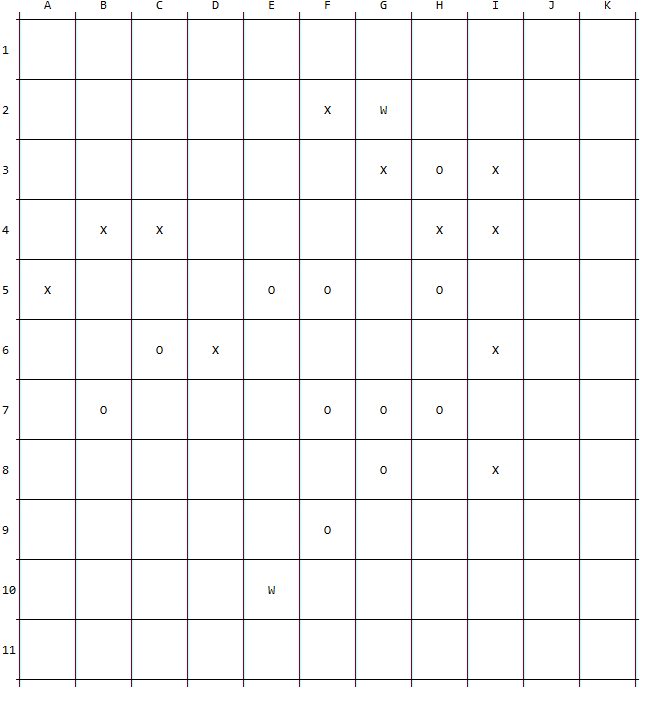
\includegraphics[height=4cm, width=4cm]{images/self_semi_board.png}
	\caption{Representação de um tabuleiro na consola}
	\label{Figura 9}
\end{center}
\end{figure}

\newpage

\subsection{Lista de Jogadas Válidas}

A obtenção da lista de jogadas é feita através do predicado \textbf{getIntersections (Board, Row1, Col1, Row2, Col2, Positions)}, que dadas as posições dos dois Trabalhadores calcula as interseções das suas linhas de visão. O cálculo das linhas de visão de um trabalhador é feito através do predicado \textbf{positionsInSight (Board, Row1, Col1, Pos1)}. Este predicado, calcula o campo de visão de um Trabalhador analisando todas as direções desda posição do Trabalhador até encontrar uma posição que não se encontra vazia.

\newpage

\subsection{Execução de Jogadas}

No início do jogo, são colocados os dois Trabalhadores nas posições iniciais, usando o predicado \textbf{setPiece(+Piece, +Row, +Col, +Board, -NewBoard)}. Este predicado coloca os Trabalhadores na posição dada desde que esta posição esteja vazia. A validade de uma jogada é sempre avaliada usando o predicado \textbf{isValidPlay (+PieceType, +Row, +Col, +Board)}.

No decorrer do jogo, cada jogada pode ser divida em duas partes distintas:  a movimentação, se o jogador assim o desejar, de um dos Trabalhadores e a colocação de uma peça no tabuleiro. Analizemos cada um destes processos em distinto:
\begin{itemize}
	\item A movimentação de um Trabalhador é feita através do predicado \textbf{moveWorker/6} que recebendo a posição tual do Trabalhador, a nova posição do Trabalhador e o tabuleiro, verifica que a nova posição se encontra vazia e move o Trabalhador para essa posição, devolvendo o tabuleiro atualizado. A movimentação da peça é feita através da colocação de uma célula vazia na posição anterior e a colocação do Trabalhador na nova posição, usando para ambas as ações o predicado \textbf {setPiece(+Piece, +Row, +Col, +Board, -NewBoard)}.
	\item A colocação de uma nova peça no tabuleiro é feita através do predicado \textbf{pieceInput/4}, que por sua vez faz uso do predicado \textbf{setPiece(+Piece, +Row, +Col, +Board, -NewBoard)}. Este predicado recebe um tipo de peça e coloca-a no tabuleiro, após verificar que a jogada é válida. No caso das peças serem pretas ou brancas, a validade da jogada passa pela posição indicada estar vazia e pela posição ser uma interseção das linhas de visão dos Trabalhadores.
\end {itemize}

\newpage

\subsection{Avaliação do Tabuleiro}

A avaliação do jogo pode ser conceptualmente divida em duas partes: a análise de sequências de peças, quer da própria cor, quer de peças adversárias; e o bloqueio de sequências de peças adversárias. As peças adversárias têm cotação negativa, enquanto as peças da mesma cor tem cotação positiva.

Na primeira fase, de forma a valorizar a realização de sequências, cada peça terá valor associado igual ao cubo da posição na sequência que ocupa. Exemplificando, uma sequência de três peças na horizontal tira respetiva valorização de: (1\textasciicircum3) + (2\textasciicircum3) + (3\textasciicircum3), ou seja, 1 + 8 + 27; enquanto uma sequência de três peças opostas teria o valor de (-1) + (-8) + (-27). Resumindo, a análise de cada peça é feita através da formula:
\begin{itemize}
	\item \textbf{ NumSequência\textasciicircum3} - para peças da mesma cor;
	\item \textbf{- (NumSequência\textasciicircum3)} - para peças adversárias;
\end{itemize}
Esta análise é feita nos quatro sentidos possíveis: horizontalmente, da esquerda para a direita; verticalmente, de cima para baixo; diagonalmente, com orientação ascendente; diagonalmente, com orientação descente.

A segunda fase, surgiu como necessidade de a peça não permitir a realização de sequências por parte do adversário. Se apenas se usasse a primeira fase de avaliação as peças nunca tentariam quebrar sequências inimigas, mas sim realizar as suas sequências. Assim, para evitar que isso aconteça, uma peça que quebre uma sequência inimiga, vale tanto como a sequência que quebra. Esta avaliação é feita analisando as peças adjacentes a cada peça da mesma cor, e, se a peça adjacente for inimiga, analisa-se a peça seguinte nessa linha, sendo que no final é adicionado o valor da sequência adversária. Exemplificando, uma sequência de três peças inimigas , a adição de uma peça que quebra esse sequência teria o valor de 1 + 4 + 27. Resumindo, a análise do bloqueio de sequências adversárias é feita através da fórmula (para cada sequência quebrada):
\begin{itemize}
	\item \textbf{(NumSequênciaAdversária\textasciicircum3) * factorDefesa}
\end{itemize}
De destacar, que após vários testes o factor de Defesa foi definido para 1 sendo este o valor que maior equilíbrio dá entre `ataque' e `defesa'.

A avaliação do tabuleiro é feita através da chamada do predicado:
\begin{itemize}
	\item \textbf{evaluateBoard(Side, Board, BoardValue)}
\end{itemize}

Que por sua vez usa os predicados:
\begin{itemize}
	\item \textbf{horizontalEvaluation(Side, Board, HorizontalValue)}
	\item \textbf{verticalEvaluation(Side, Board, VerticalValue)}
	\item \textbf{diagonalEvaluation(Side, Board, DiagonalValue)}
	\item \textbf{defensiveEvaluation(Side, Board, DefensiveValue)}
\end{itemize}

\newpage

\subsection{Final do Jogo} Verificação do fim do jogo, com identificação do vencedor. Exemplo: \textit{game\_over(+Board, -Winner)}.

Existem três maneiras possíveis de terminação do jogo: a inexistência  de posições que sejam a interseção da linha de visão dos Trabalhadores; o tabuleiro estar cheio e não ser possível mover um Trabalhador; a existência de cinco em linha de um tipos de peças.
Assim, internamente, a verificação destas condições é feita de três formas distintas:
\begin{itemize}
	\item No caso de uma jogada feita pelo utilizador, após a colocação dos Trabalhadores no tabuleiro é verificado se é possível a execução de uma jogada, recorrendo ao predicado \textbf{isPiecePlayPossible(Board)}, que verifica se a interseção das linhas de visão dos dois trabalhadores não é uma lista vazia. Caso a lista seja vazia, a primeira declaração do predicado \textbf{gameLoop}, que controla o ciclo de jogo, falhará, realizando assim a segunda declaração, que declara vitorioso o adversário e termina o ciclo de jogo. No caso de uma jogada controlada automaticamente, caso a lista dos tabuleiros possíveis, correspondentes a uma jogada, seja vazia, é declarada a vitória do adversária, num processo semelhante ao executado para o jogador.
	\item No início de cada jogada é verificado a se o tabuleiro se encontra totalmente preenchido, não sendo assim possível mexer \textit{workers} ou posicionar peças. Esta verificação é realizada através do predicado \textbf{boardIsNotFull(Board)}, que itera pelo tabuleiro até encontrar uma posição vazia. Caso não seja possível, a primeira declaração do ciclo de jogo falha e, à semelhança do ponto anterior, o jogador adversário é declarado vitorioso.
	\item No final de cada jogada, é verificada a vitória desse jogador. Para tal, o predicado \textbf{decideNextStep} chama o predicado \textbf{gameIsWon(Side, Board)}, que, fazendo uso dos predicados \textbf{checkHorizontalWin(PieceSide, Board)}, \textbf{checkVerticalWin(PieceSide, Board)} e \textbf{checkDiagonalWin (PieceSide, Board)}, verifica se existem 5 peças em linha, significando assim a vitória do jogador atual. Caso nenhum destes predicados se verifique, o predicado \textbf{decideNextStep} volta a chamar o ciclo do jogo, par ao próximo jogador.
\end{itemize}

\newpage

\subsection{Jogada do Computador} Escolha da jogada a efetuar pelo computador, dependendo do nível de dificuldade. Por exemplo: \textit{choose\_move(+Level, +Board, -Move)}.

\newpage

%%%%%%%%%%%%%%%%%%%%%%%%%%
\section{Interface com o Utilizador}

A interface do utilizador foi feita de forma a ser resiliente a \textit{Input} e a permitir que o jogo nunca acaba abruptamente. É visualmente agradável e simples, melhor a experiência de jogo para o utilizador. As funções usadas na interface encontram-se maioritariamente definidas nos ficheiros \textbf{input.pl}, \textbf{display.pl} e \textbf{menus.pl}.

\begin{figure}[h!]
\begin{center}
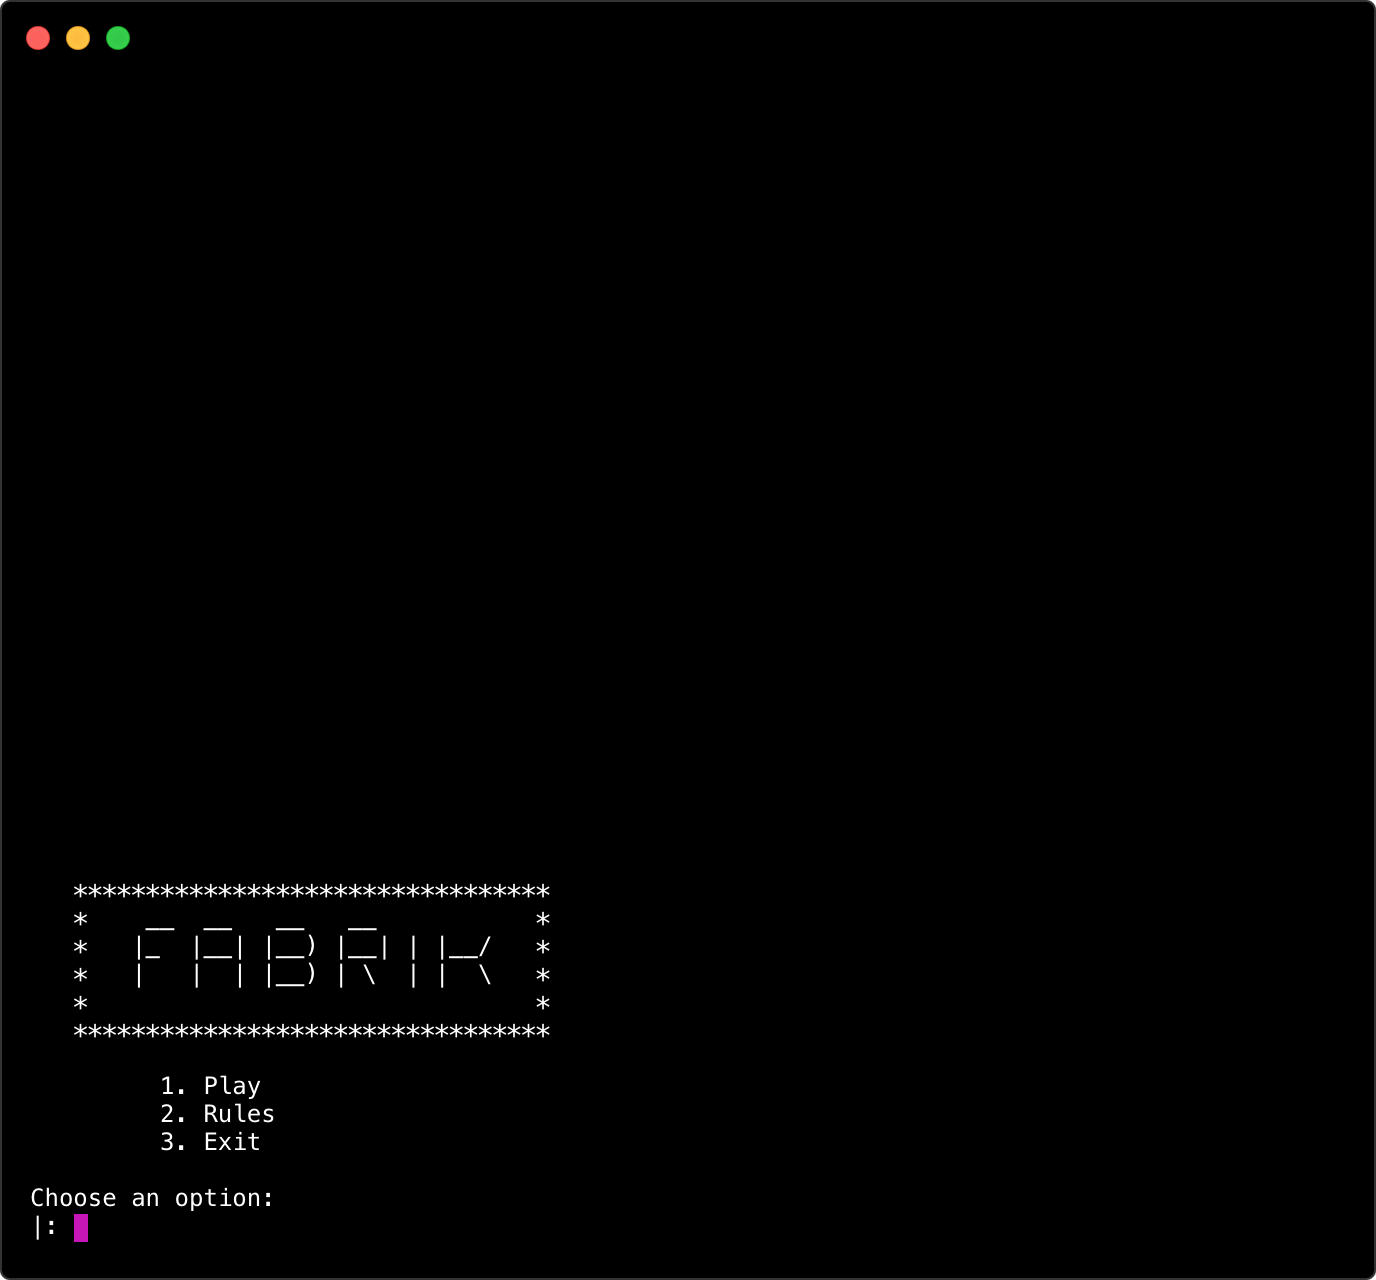
\includegraphics[height=7cm,width=7cm]{images/fabrik_start.png}
\caption{Menu Prinicipal}
\label{Figura 1}
\end{center}
\end{figure}

\begin{figure}[h!]
\begin{center}
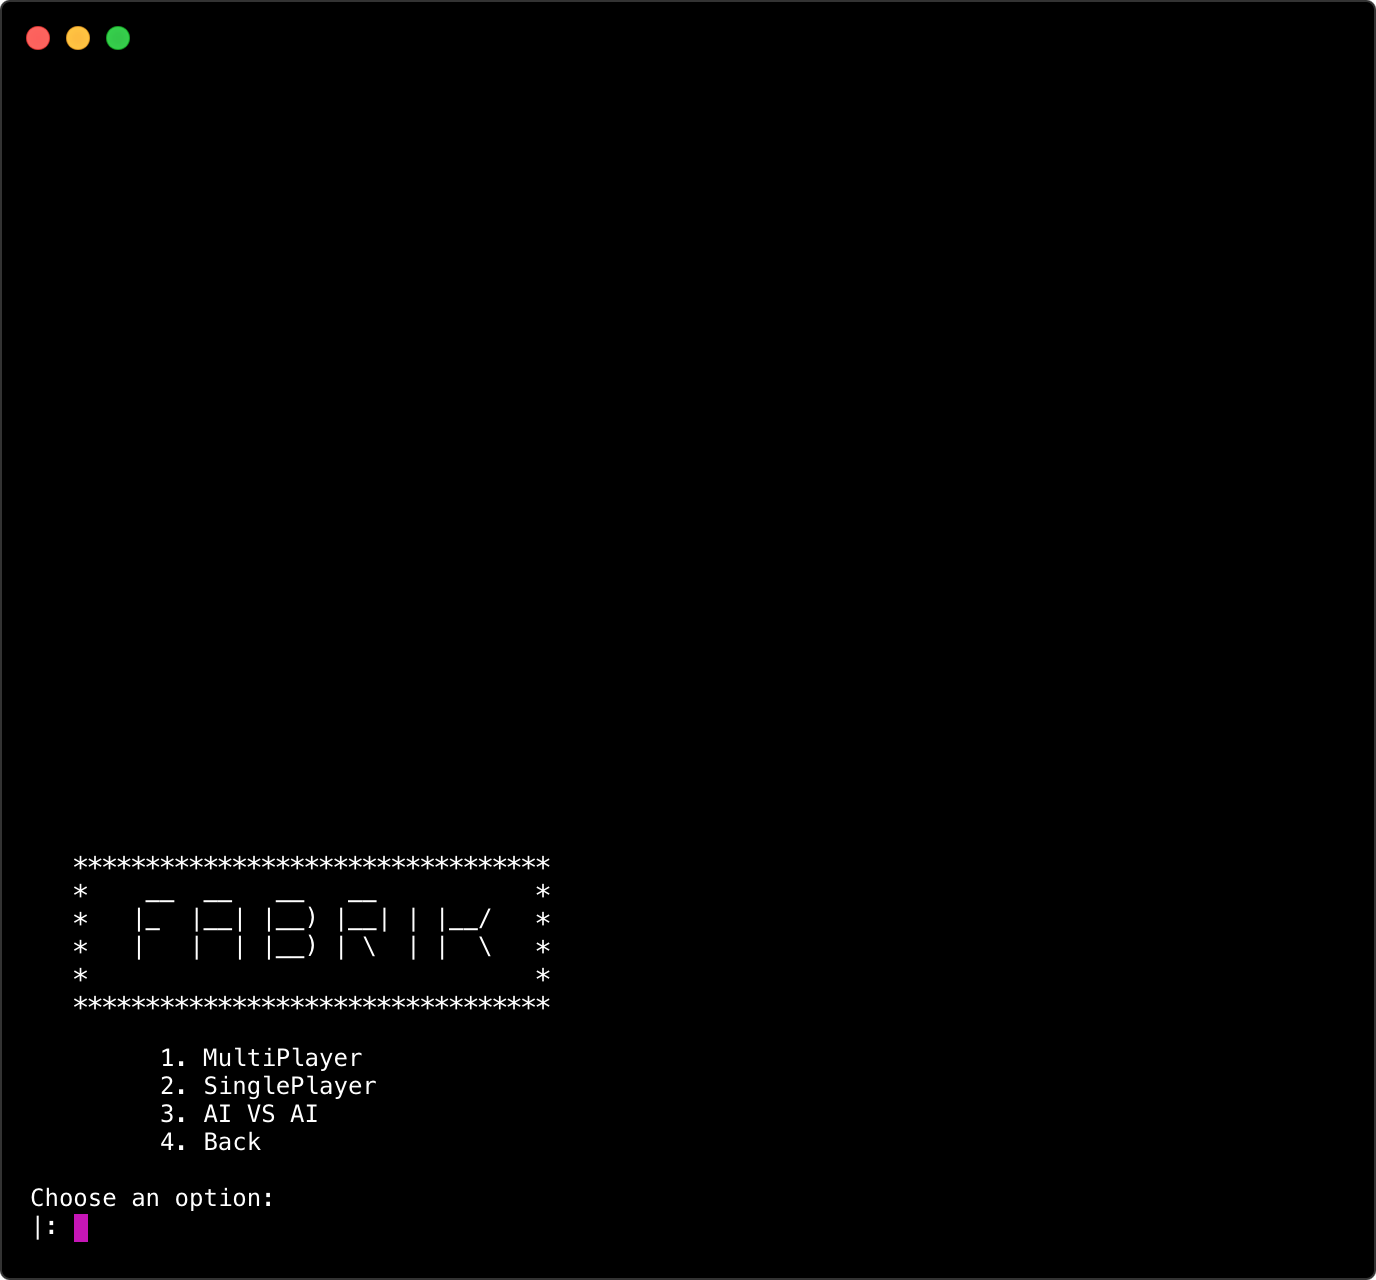
\includegraphics[height=7cm,width=7cm]{images/fabrik_menu.png}
\caption{Menu de Jogo}
\label{Figura 1}
\end{center}
\end{figure}

\begin{figure}[h!]
\begin{center}
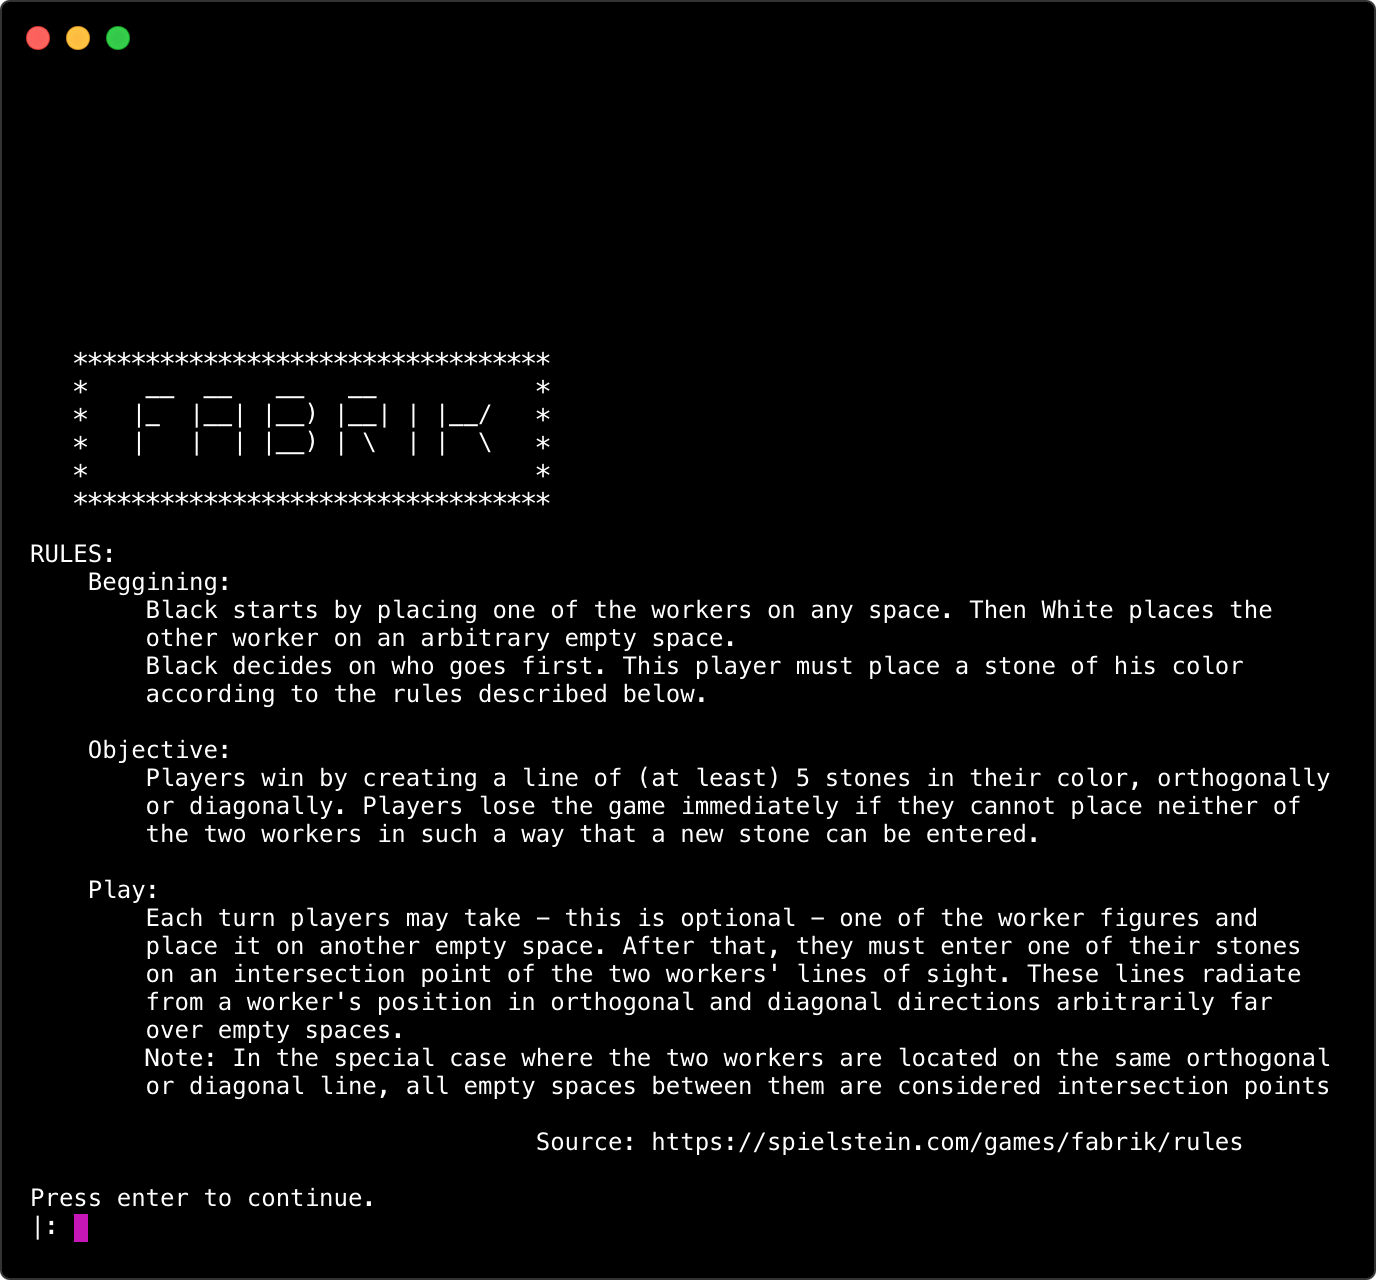
\includegraphics[height=7cm,width=7cm]{images/fabrik_rules.png}
\caption{Regras}
\label{Figura 1}
\end{center}
\end{figure}

\begin{figure}[h!]
\begin{center}
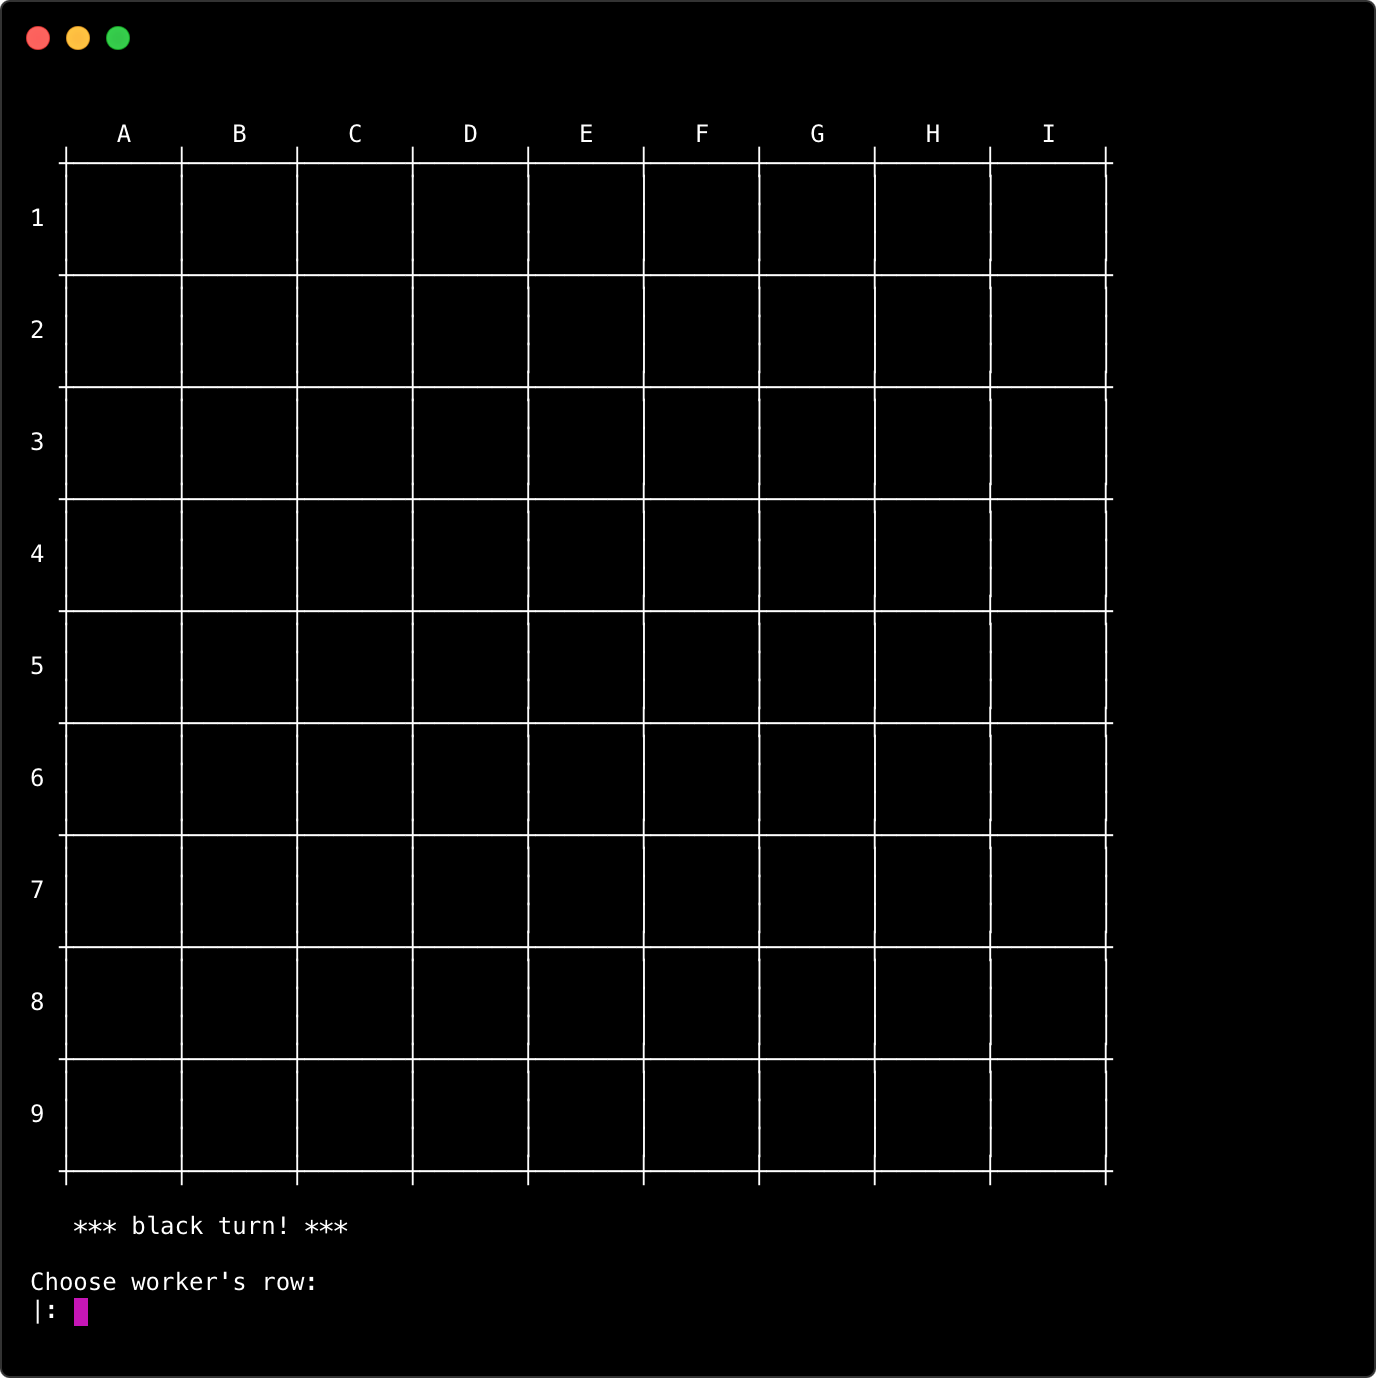
\includegraphics[height=7cm,width=7cm]{images/fabrik_choose_worker.png}
\caption{Colocação de um Trabalhador}
\label{Figura 1}
\end{center}
\end{figure}

\begin{figure}[h!]
\begin{center}
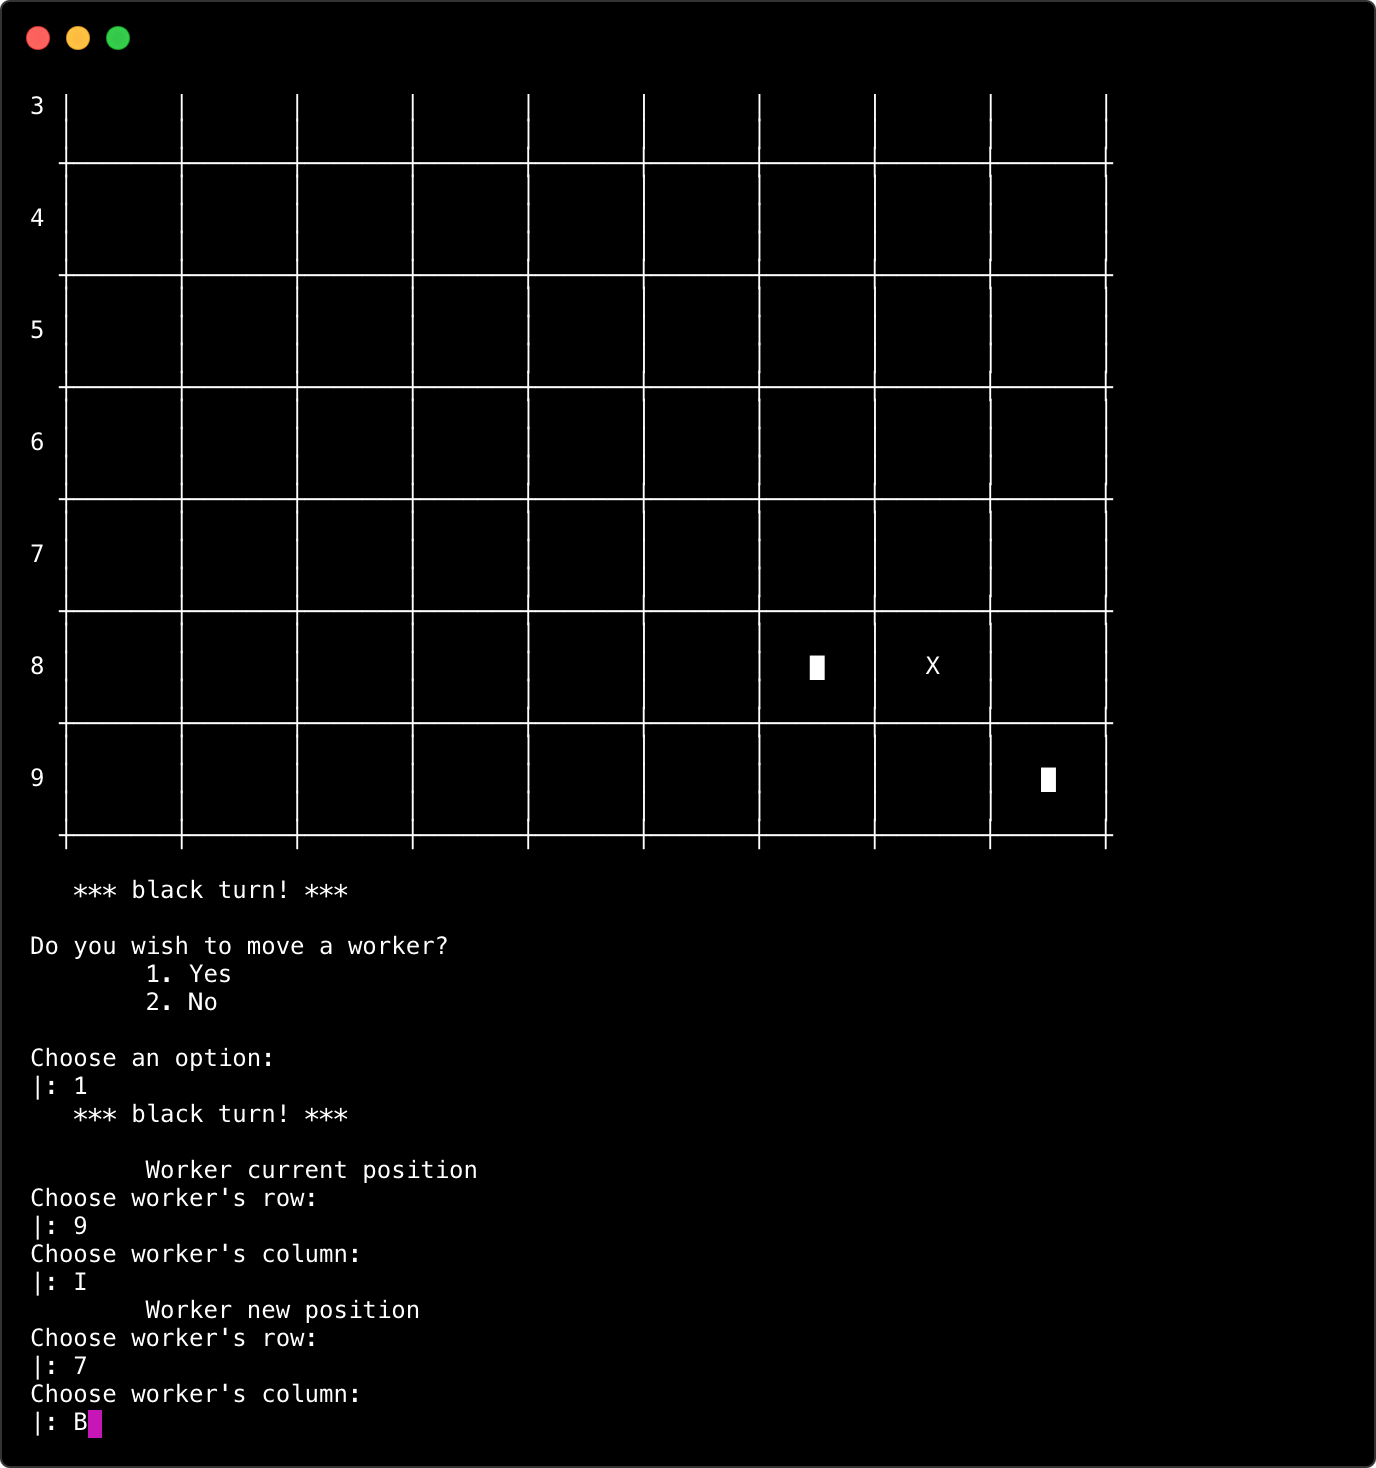
\includegraphics[height=7cm,width=7cm]{images/fabrik_change_worker_pos.png}
\caption{Movimentação de um trabalhador}
\label{Figura 1}
\end{center}
\end{figure}

\begin{figure}[h!]
\begin{center}
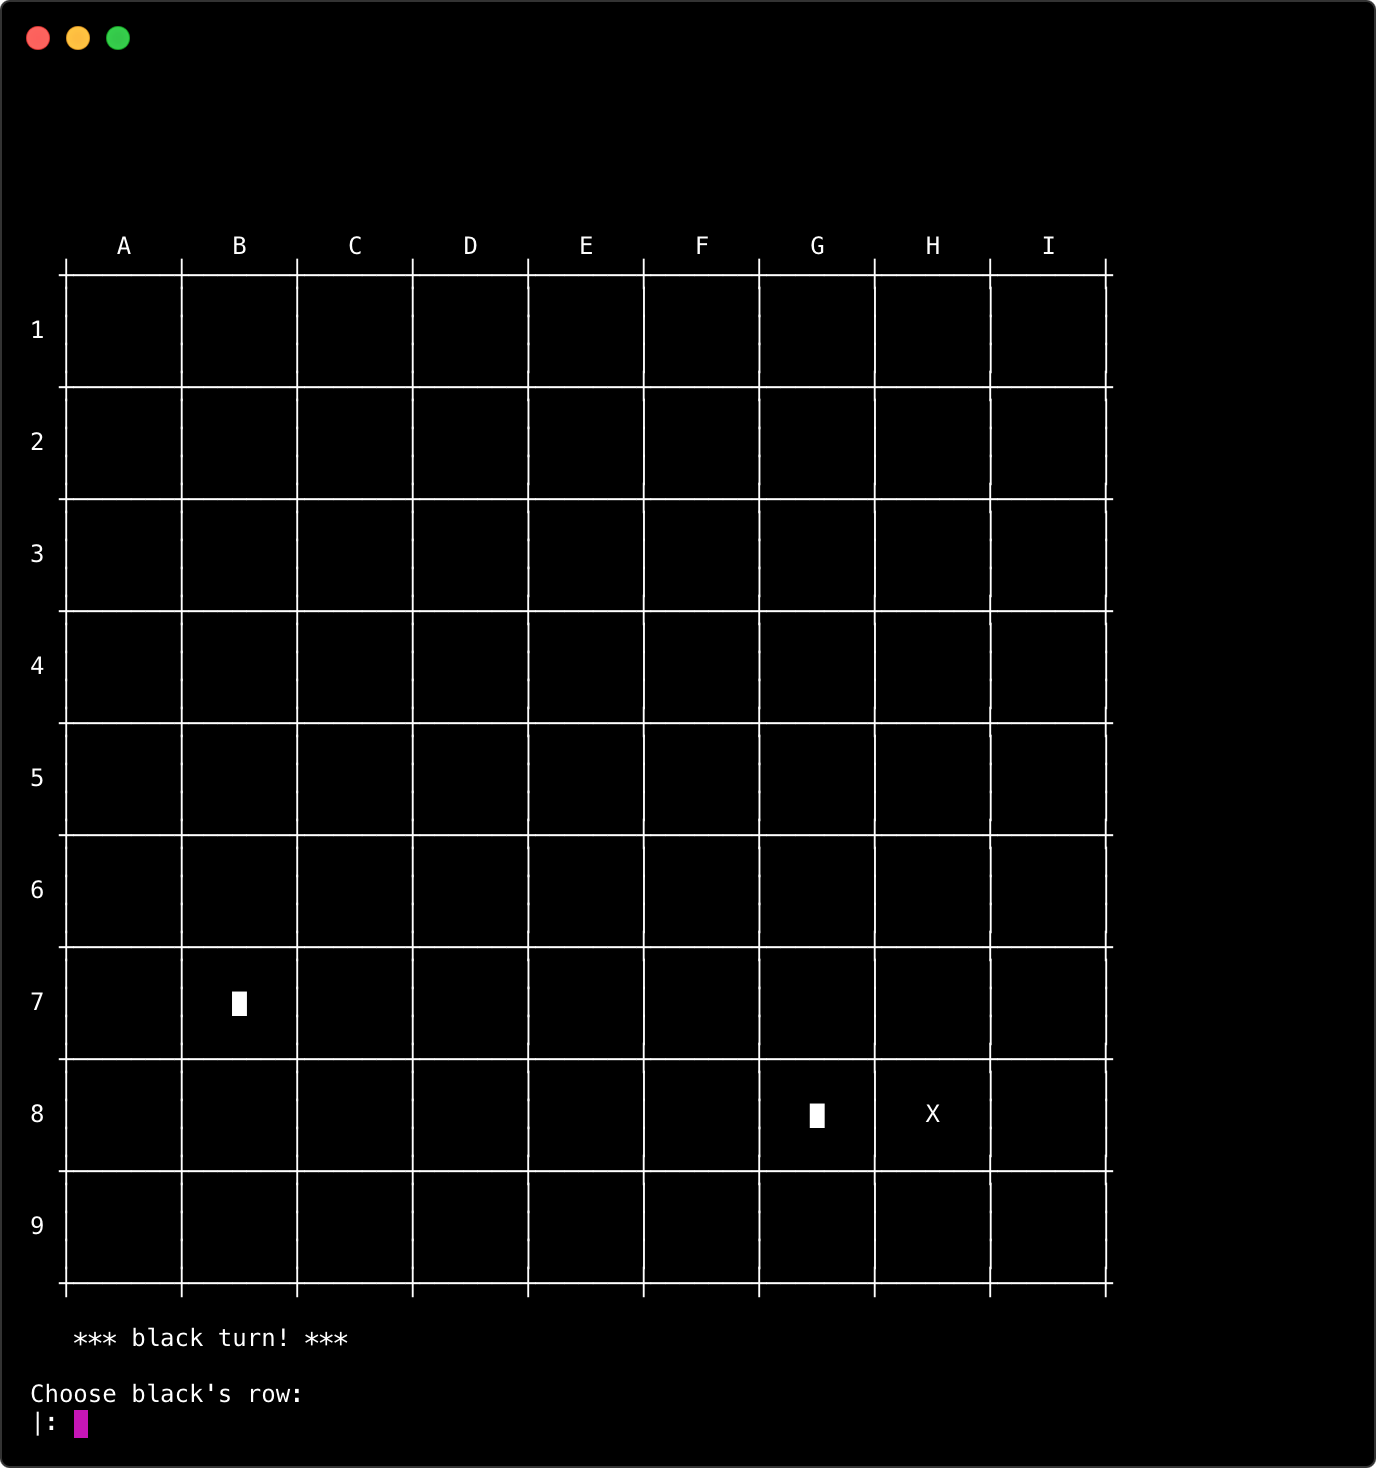
\includegraphics[height=7cm,width=7cm]{images/fabrik_set_piece.png}
\caption{Colocação de um Peça}
\label{Figura 1}
\end{center}
\end{figure}

\clearpage
\newpage
\newpage

%%%%%%%%%%%%%%%%%%%%%%%%%%
\section{Conclusões}
O presente trabalho exigiu um grande empenho por parte de ambos os elementos do grupo, tendo, no entanto, sido uma experiência recompensadora.

Consideramos que o nosso conhecimento de programação em lógica foi amplamente aumentado, tendo sido alcançado tudo o que nos propusemos a fazer no tempo requerido, e muitas vezes ultrapassado por termos encontrado soluções mais interessantes.

As maiores dificuldades encontradas no decorrer do desenvolvimento foram relacionadas com a verificação das jogadas válidas (pois o jogo impõe múltiplas restrições a esta ação), assim como na elaboração da função que avalia as jogadas possíveis. No entanto, todos os problemas foram eventualmente ultrapassados, e estamos contentes com as soluções encontradas.

Achamos importante indicar que próximo do fim do desenvolvimento tentamos aplicar o algoritmo \textit{Minimax} para a tomada de decisão sobre a melhor jogada a escolher, no entanto tornou-se eventualmente claro que, devido às custosas verificações de validade de jogadas e de fim de jogo, esta alteração implicaria um grande tempo de espera para cada jogada do computador, tendo no fim sido escolhido um algoritmo ganancioso para a referida tomada de decisão.

Referir também que em alguns casos decidimos beneficiar legibilidade em detrimento de performance, privilegiando predicados curtos e com uso de funções \textit{standard}, mantendo a elegância de código permitida em linguagens de alto nível como o \textit{PROLOG}.

Em suma, apesar de \textit{PROLOG} se pautar por um paradigma diferente do que estamos habituados, rápidamente nos habituamos e aprendemos a apreciar as facilidades e dificuldades que este apresenta, tendo culminado num trabalho no qual nos orgulhamos.


\clearpage
\addcontentsline{toc}{section}{Bibliografia}
\renewcommand\refname{Bibliografia}
\bibliography{myrefs}
\bibliographystyle{ieeetr}


\newpage
\appendix
\section{Código Comentado}

\huge\textbf{fabrik.pl}
\begin{lstlisting}
:- include('board.pl').
:- include('display.pl').
:- include('utils.pl').
:- include('menus.pl').
:- include('input.pl').
:- include('ai.pl').
:- include('test.pl').
:- use_module(library(random)).


fabrik:-
	mainMenuHandler.

%Game Initialization - set Workers and choose who starts
initGame(Player1, Player2) :-
	genRowColFacts,
	boardSize(N), !,
	createBoard(B0, N), printBoard(B0),
	setFirstWorker(Player1, black, B0, B1), printBoard(B1),
	setFirstWorker(Player2, black, B1, B2), printBoard(B2),
	chooseStartingPlayer(Player1, Side), printBoard(B2), !,
	gameLoop(Player1, Player2, Side, B2).
%If somehting failed on initGame, return to Play Menu
initGame(_, _):-
	playMenuHandler.

%game Loop for Player 1
gameLoop(Player1Function, Player2Function, black, Board) :-
	boardIsNotFull(Board),
	call(Player1Function, black, Board, NewBoard), printBoard(NewBoard),
	decideNextStep(Player1Function, Player2Function, black, NewBoard), !.
%Player 1 could not place a piece, so he lost
gameLoop(_Player1Function, _Player2Function, black, _Board) :- victory(white), !.

%game Loop for Player 2
gameLoop(Player1Function, Player2Function, white, Board) :-
	boardIsNotFull(Board),
	call(Player2Function, white, Board, NewBoard), printBoard(NewBoard),
	decideNextStep(Player1Function, Player2Function, white, NewBoard), !.
%Player 2 could not place a piece, so he lost
gameLoop(_Player1Function, _Player2Function, white, _Board) :- victory(black), !.


%Decide If someone has won with N in a row, or if the game should progress
decideNextStep(_Player1Function, _Player2Function, Side, Board) :-
	gameIsWon(Side, Board), !,
	victory(Side).
decideNextStep(Player1Function, Player2Function, Side, Board) :-
	changePlayer(Side, NewSide), !,
	gameLoop(Player1Function, Player2Function, NewSide, Board).

%End game with victory of Side
victory(Side):-
	destroyRowColFacts, !,
	wonMsg(Side),
	getEnter, !.

%Executes a human Play, getting worker input and piece input
humanPlay(Side, Board, NewBoard) :-
	workerUpdate(Side, Board, TempBoard),
	printBoard(TempBoard),
	isPiecePlayPossible(TempBoard), !,
	pieceInput(Side, Side, TempBoard, NewBoard), !.

%Setting the First Workers on the Board - Game beggining
setFirstWorker('humanPlay', Side, Board, NewBoard) :-
	pieceInput(worker, Side, Board, NewBoard).
%For AI Functions
setFirstWorker(_, _Side, Board, NewBoard) :-
        boardSize(Size),
        random(0, Size, Row), random(0, Size, Col),
        setPiece(worker, Row, Col, Board, NewBoard).

%Choose the Player that starts putting pieces on the board
chooseStartingPlayer('humanPlay', Side) :-
        getFirstPlayer(Side), !.
chooseStartingPlayer(_, white). % always white - For AI functions 
\end{lstlisting}
\newpage

\huge\textbf{board.pl}
\begin{lstlisting}
:- use_module(library(lists)).
:- use_module(library(clpfd)).
:- use_module(library(sets)).

% Generate a board predicate with N x N empty spaces
createBoard(Board, N) :-
        createBoard(Board, N , 0).

createBoard(_, N, N).
createBoard([FirstRow | OtherRows], N, Lines) :-
        Lines1 is (Lines + 1),
        createBoardLine(FirstRow, N),
        createBoard(OtherRows, N, Lines1).
        
createBoardLine(_, 0).
createBoardLine([FirstEle | OtherEle], N) :-
        FirstEle = none,
        N1 is (N - 1),
        createBoardLine(OtherEle, N1).


% Access the element in the [Row,Col] position of the given board
getElement(Board, Row, Col, Element):-
        nth0(Row, Board, RowLine, _),
        nth0(Col, RowLine, Element, _), !.


%% Validation Predicates
% Worker can be played if [Row,Col]=none
isValidPlay(worker, Row, Col, Board) :- !,
        getElement(Board, Row, Col, none).

% No conditions if there is no piece
isValidPlay(none, _, _, _) :- !.

% White/Black pieces can be played if [Row,Col] is in intersection of Workers' lines of sight
isValidPlay(_, Row, Col, Board) :-
        getElement(Board, Row, Col, none),
        isIntersection(Board, Row, Col).

% Fetches the position of both workers and checks if [Row,Col] is in their lines of sight
isIntersection(Board, Row, Col) :-
        findBothWorkers(Board, Row1, Col1, Row2, Col2),
        getIntersections(Board, Row1, Col1, Row2, Col2, Positions),
        member([Row, Col], Positions).

% Gets the intersections of the workers' lines of sight
getIntersections(Board, Row1, Col1, Row2, Col2, Positions) :-
        positionsInSight(Board, Row1, Col1, Pos1),
        positionsInSight(Board, Row2, Col2, Pos2),
        intersection(Pos1, Pos2, Positions).

% Position is in Board and is empty ?
isValidPosition(Board, Row, Col) :-
        boardSize(N),
        Row >= 0, Col >= 0,
        Row =< N, Col =< N,
        getElement(Board, Row, Col, none).

% Possible values for coordinates' change
coordinateChange(0).
coordinateChange(1).
coordinateChange(-1).

rowColChange(RowChange, ColChange) :-
        coordinateChange(RowChange),
        coordinateChange(ColChange),
        \+ (RowChange = 0, ColChange = 0).

% Spreads outwards from the worker's position and stops on end of board or when a piece blocks the line of sight
% Returns all positions of the worker's lines of sight
positionsInSight(Board, Row, Col, Positions) :-
        findall(PartialPositions, (rowColChange(RChange,CChange), lineOfSight(Board, Row, Col, RChange, CChange, PartialPositions)), ListOfLists),
        append(ListOfLists, Positions).

lineOfSight(Board, Row, Col, RowChange, ColChange, Positions) :-
        NewRow is Row + RowChange, NewCol is Col + ColChange,
        isValidPosition(Board, NewRow, NewCol), !,
        lineOfSight(Board, NewRow, NewCol, RowChange, ColChange, OtherPositions),
        append([[NewRow, NewCol]], OtherPositions, Positions).
lineOfSight(_Board, _Row, _Col, _RowChange, _ColChange, []) :- !.

                                                                   
% Set piece on board
% Sets the piece of the given type on the given position, on the given Board
setPiece(Piece, Row, Col, Board, NewBoard) :-
        isValidPlay(Piece, Row, Col, Board),
        nth0(Row, Board, RowLine, TmpBoard),
        nth0(Col, RowLine, _, TmpRowLine),
        nth0(Col, NewRowLine, Piece, TmpRowLine),
        nth0(Row, NewBoard, NewRowLine, TmpBoard).


% Finds both workers' positions
findBothWorkers(Board, Row1, Col1, Row2, Col2) :-
        findWorker(Board, Row1, Col1),
        findWorker(Board, Row2, Col2),
        \+ (Row1 = Row2, Col1 = Col2), !. % Cut prevents backtracking over Row/Col permutations 

% Finds a worker's position
findWorker(Board, OutputRow, OutputCol) :-
        nth0(OutputRow, Board, TmpRow),
        nth0(OutputCol, TmpRow, worker).

% Tests if board has any empty space
boardIsNotFull(Board) :-
        nth0(_, Board, TmpRow),
        nth0(_, TmpRow, none).

% Side has won ?
gameIsWon(PieceSide, Board):-
        checkHorizontalWin(PieceSide, Board).
gameIsWon(PieceSide, Board):-
        checkVerticalWin(PieceSide, Board).
gameIsWon(PieceSide, Board):-
        checkDiagonalWin(PieceSide, Board).

% Check Horizontal Win for side 'Side'
checkHorizontalWin(Side, [FirstRow | _RestOfBoard]) :-
        checkRowWin(Side, FirstRow, 0).
checkHorizontalWin(Side, [FirstRow | RestOfBoard]) :-
        \+ checkRowWin(Side, FirstRow, 0),
        checkHorizontalWin(Side, RestOfBoard).
checkRowWin(_, _, N) :-
        winningStreakN(N), !.
checkRowWin(Side, [Side | RestOfRow], Count) :-
        NewCount is Count + 1,
        checkRowWin(Side, RestOfRow, NewCount).
checkRowWin(Side, [FirstEl | RestOfRow], _Count) :-
        Side \= FirstEl,
        checkRowWin(Side, RestOfRow, 0).


% Check Vertical Win for side 'Side'
checkVerticalWin(Side, Board) :-
        transpose(Board, TransposedBoard),
        checkHorizontalWin(Side, TransposedBoard).

%Check Diagonal Win for side 'Side'
checkDiagonalWin(Side, Board):-
        boardSize(BoardSize),
        checkDiagWinAux(Side, Board, 0, BoardSize).

%One quarter of the diagonal lines: left-right, top-down
checkDiagWinAux(Side, Board, Col, _BoardSize):-
        checkDiagLineWin(Side, Board, 0, Col, 1, 1, 0).
%One quarter of the diagonal lines: right-left, top-down
checkDiagWinAux(Side, Board, Col, _BoardSize):-
        checkDiagLineWin(Side, Board, 0, Col, 1, -1, 0).
%One quarter of the diagonal lines: left-right, down-top
checkDiagWinAux(Side, Board, Col, BoardSize):-
        BottomRow is (BoardSize - 1),
        checkDiagLineWin(Side, Board, BottomRow, Col, -1, 1, 0).
%One quarter of the diagonal lines: right-left, down-top
checkDiagWinAux(Side, Board, Col, BoardSize):-
        BottomRow is (BoardSize - 1),
        checkDiagLineWin(Side, Board, BottomRow, Col, -1, -1, 0).
%Recursive Call
checkDiagWinAux(Side, Board, Col, BoardSize):-
        NewCol is (Col + 1),
        NewCol \= BoardSize,
        checkDiagWinAux(Side, Board, NewCol, BoardSize).

%Iterates through the diagonal line, starting at [Row, Col], with direction Vector [RowInc, ColInc], checking for Winning Streak
%Found N in-a-row, won game!
checkDiagLineWin(_Side, _Board, _Row, _Col, _RowInc, _ColInc, Count):-
        winningStreakN(Count), !.
checkDiagLineWin(Side, Board, Row, Col, RowInc, ColInc, Count):-
        getElement(Board, Row, Col, Side),
        NewRow is (Row + RowInc), NewCol is (Col + ColInc),
        NewCount is (Count + 1),
        checkDiagLineWin(Side, Board, NewRow, NewCol, RowInc, ColInc, NewCount).
checkDiagLineWin(Side, Board, Row, Col, RowInc, ColInc, _Count):-
        getElement(Board, Row, Col, _),
        NewRow is (Row + RowInc), NewCol is (Col + ColInc),
        checkDiagLineWin(Side, Board, NewRow, NewCol, RowInc, ColInc, 0).

%Moves a worker from the position [Row, Col] to the position [DestRow, DestCol], if possible
moveWorker(Board, Row, Col, DestRow, DestCol, UpdatedBoard):-
        getElement(Board, Row, Col, worker),
        setPiece(none, Row, Col, Board, TempBoard),
        setPiece(worker, DestRow, DestCol, TempBoard, UpdatedBoard).

% Checks if any play is possible (with the worker already having been placed)
isPiecePlayPossible(Board) :-
        findBothWorkers(Board, R1, C1, R2, C2),
        getIntersections(Board, R1, C1, R2, C2, PossiblePlays),
        length(PossiblePlays, Length),
        Length > 0, !.
\end{lstlisting}
\newpage

\huge\textbf{ai.pl}
\begin{lstlisting}
:- use_module(library(random)).
:- dynamic(validCoord/1).

% Defense factor in AI evaluation function
defenseFactor(Value, NewValue):-
	NewValue is (Value * 1).

%Destroy the board facts generated for every game
destroyRowColFacts:-
	retractall(validCoord(_)). 

% Possible values for Row and Col positions
genRowColFacts:-
	boardSize(N),
	genRowColFactsAux(0, N), !.

genRowColFactsAux(Current, Current).
genRowColFactsAux(Current, BoardSize) :-
	asserta(validCoord(Current)),
	NewValue is (Current + 1),
	genRowColFactsAux(NewValue, BoardSize).

% Used to backtrace over the possible positions
validCoordinates(RowChange, ColChange) :-
        validCoord(RowChange),
        validCoord(ColChange).

% returns a List containing all the possible Boards by moving the workers
getAllWorkerPermutations(Board, PossibleBoards) :-
	findBothWorkers(Board, Row1, Col1, Row2, Col2),
	getWorkerBoards(Board, Row1, Col1, PossibleBoards1),
	getWorkerBoards(Board, Row2, Col2, PossibleBoards2),
	union(PossibleBoards1, PossibleBoards2, PossibleBoards). % No duplicates

% All the boards obtained by moving a worker through a Board
getWorkerBoards(Board, Row, Col, ListOfBoards) :-
	findall(PossibleBoard, (validCoordinates(NewRow, NewCol), moveWorker(Board, Row, Col, NewRow, NewCol, PossibleBoard)), ListOfBoards), !.

% Get all the boards where a piece can go, given a List of Boards with different worker positions
getPieceBoards(Side, WorkerBoards, PossibleBoards) :-
	getPieceBoardsAux(Side, WorkerBoards, [], PossibleBoards).

getPieceBoardsAux(_, [], PossibleBoards, PossibleBoards) :- !.
getPieceBoardsAux(Side, [WorkerBoard | OtherBoards], SoFarBoards, PossibleBoards) :-
	findBothWorkers(WorkerBoard, Row1, Col1, Row2, Col2),
	getIntersections(WorkerBoard, Row1, Col1, Row2, Col2, IntersectionsList),
	genNewBoards(Side, WorkerBoard, IntersectionsList, [], NewBoards),
	append(NewBoards, SoFarBoards, UpdatedBoards), !,
	getPieceBoardsAux(Side, OtherBoards, UpdatedBoards, PossibleBoards).

% Generates all the boards associated to a certain board with fix workers.
% Boards with all the different places where the piece can be played
genNewBoards(_, _, [], AllBoards, AllBoards) :- !.
genNewBoards(Side, Board, [Intersec | OtherIntersec], FoundBoards, AllBoards) :-
	Intersec = [Row, Col],
	setPiece(Side, Row, Col, Board, TempBoard),
	append([TempBoard], FoundBoards, UpdatedBoards), !,
	genNewBoards(Side, Board, OtherIntersec, UpdatedBoards, AllBoards).

% Returns all the possible resulting boards, taking into account the move worker play and the set piece play
getPossibleBoards(Side, Board, PossibleBoards) :-
	getAllWorkerPermutations(Board, WorkerBoards), !,
	getPieceBoards(Side, WorkerBoards, PossibleBoards),
	length(PossibleBoards, Size),
	Size > 0. %If no board is created, game is Over


% Evaluates a board and returns the correspondent Value
evaluateBoard(Side, Board, BoardValue) :-
	horizontalEvaluation(Side, Board, HorizontalValue),
	verticalEvaluation(Side, Board, VerticalValue),
	diagonalEvaluation(Side, Board, DiagonalValue),
	defensiveEvaluation(Side, Board, DefensiveValue),
	BoardValue is (HorizontalValue + VerticalValue + DiagonalValue + DefensiveValue).

% Makes an Horizontal Evaluation of the given board
horizontalEvaluation(Side, Board, Value) :-
	horizontalEvaluationAux(Side, Board, 0 , Value), !.
horizontalEvaluationAux(_, [], FinalValue, FinalValue) :- !.
horizontalEvaluationAux(Side, [FirstRow | RestOfBoard], CurrentValue, FinalValue) :-
	horizontalRowEvaluation(Side, FirstRow, 0, 0, CurrentValue, LineFValue),
	horizontalEvaluationAux(Side, RestOfBoard, LineFValue, FinalValue).

horizontalRowEvaluation(_, [], _, _, LineFValue, LineFValue) :- !.
% Succession of Side Pieces
horizontalRowEvaluation(Side, [Side | OtherCols], Streak, _EnemyStreak, CurrentValue, LineFValue) :-
	NewStreak is (Streak + 1),
	NewValue is (CurrentValue + (NewStreak * NewStreak * NewStreak)),
	% neighborEnemyStreaks
	horizontalRowEvaluation(Side, OtherCols, NewStreak, 0, NewValue, LineFValue).
% Succession of Enemy Pieces
horizontalRowEvaluation(Side, [Col | OtherCols], _Streak, EnemyStreak, CurrentValue, LineFValue) :-
	changePlayer(Side, Enemy),
	Col = Enemy,
	NewEnemyStreak is (EnemyStreak + 1),
	NewValue is (CurrentValue - (NewEnemyStreak * NewEnemyStreak * NewEnemyStreak)),
	horizontalRowEvaluation(Side, OtherCols, 0, NewEnemyStreak, NewValue, LineFValue).
% When nor white nor black
horizontalRowEvaluation(Side, [_Col | OtherCols], _, _, CurrentValue, Value) :-
	horizontalRowEvaluation(Side, OtherCols, 0, 0, CurrentValue, Value).

% Makes a vertical Evaluation of the given board
verticalEvaluation(Side, Board, Value) :-
	transpose(Board, TransposedBoard),
	horizontalRowEvaluation(Side, TransposedBoard, 0, 0, 0, Value).

% Makes a diagonal Evaluation of the given board
diagonalEvaluation(Side, Board, Value) :-
	boardSize(BoardSize),
	diagonalEvaluationAux(Side, Board, 0, BoardSize, 0, Value).
diagonalEvaluationAux(_Side, _Board, BoardSize, BoardSize, FinalValue, FinalValue) :- !.
diagonalEvaluationAux(Side, Board, Col, BoardSize, CurrentValue, Value) :-
	BottomRow is (BoardSize - 1),
	ColWithoutMainDiag is (Col - 1),
	% One quarter of the diagonal lines: left-right, top-down
	diagonalLine(Side, Board, 0, Col, 1, 1, 0, 0, CurrentValue, DiagLine1Value),
	% One quarter of the diagonal lines: right-left, top-down
	diagonalLine(Side, Board, 0, ColWithoutMainDiag, 1, -1, 0, 0, DiagLine1Value, DiagLine2Value),
	% One quarter of the diagonal lines: left-right, down-top
	diagonalLine(Side, Board, BottomRow, Col, -1, 1, 0, 0, DiagLine2Value, DiagLine3Value),
	% One quarter of the diagonal lines: right-left, down-top
	diagonalLine(Side, Board, BottomRow, ColWithoutMainDiag, -1, -1, 0, 0, DiagLine3Value, DiagLine4Value),
	NewCol is (Col + 1),
	diagonalEvaluationAux(Side, Board, NewCol, BoardSize, DiagLine4Value, Value).

% Iterates thorugh the diagonal line, starting at [Row, Col] with the direction Vector [RowInc, ColInc], updating the line value
% Succession of Side Pieces
diagonalLine(Side, Board, Row, Col, RowInc, ColInc, Streak, _EnemyStreak, CurrentValue, FinalValue) :-
	getElement(Board, Row, Col, Side),
	NewRow is (Row + RowInc), NewCol is (Col + ColInc),
	NewStreak is (Streak + 1),
	NewValue is (CurrentValue + (NewStreak * NewStreak * NewStreak)),
	diagonalLine(Side, Board, NewRow, NewCol, RowInc, ColInc, NewStreak, 0, NewValue, FinalValue).
% Sucession of Enemy Pieces
diagonalLine(Side, Board, Row, Col, RowInc, ColInc, _Streak, EnemyStreak, CurrentValue, FinalValue) :-
	changePlayer(Side, Enemy),
	getElement(Board, Row, Col, Enemy),
	NewRow is (Row + RowInc), NewCol is (Col + ColInc),
	NewEStreak is (EnemyStreak + 1),
	NewValue is (CurrentValue - (NewEStreak * NewEStreak * NewEStreak)),
	diagonalLine(Side, Board, NewRow, NewCol, RowInc, ColInc, 0, NewEStreak, NewValue, FinalValue).
% When nor white nor black
diagonalLine(Side, Board, Row, Col, RowInc, ColInc, _Streak, _EnemyStreak, CurrentValue, FinalValue) :-
	getElement(Board, Row, Col, _),
	NewRow is (Row + RowInc), NewCol is (Col + ColInc),
	diagonalLine(Side, Board, NewRow, NewCol, RowInc, ColInc, 0, 0, CurrentValue, FinalValue).
% It only fails again if [Row, Col] out of board
diagonalLine(_Side, _Board, _Row, _Col, _RowInc, _ColInc, _Streak, _EnemyStreak, FinalValue, FinalValue) :- !.


defensiveEvaluation(Side, Board, Value) :-
	defensiveEvaluationRec(Side, Board, 0, 0, 0, Value).
% Piece is of type Side
defensiveEvaluationRec(Side, Board, Row, Col, CurrentValue, Value) :-
	getElement(Board, Row, Col, Side),
	updateDefenseValue(Side, Board, Row, Col, CurrentValue, UpdatedValue),
	getNextPosition(Row, Col, NewRow, NewCol),
	defensiveEvaluationRec(Side, Board, NewRow, NewCol, UpdatedValue, Value).
% Piece is not of type Side
defensiveEvaluationRec(Side, Board, Row, Col, CurrentValue, Value) :-
	getElement(Board, Row, Col, _),
	getNextPosition(Row, Col, NewRow, NewCol),
	defensiveEvaluationRec(Side, Board, NewRow, NewCol, CurrentValue, Value).
% Finished, accessed non-existent element - Finished Board
defensiveEvaluationRec(_, _, _, _, FinalValue, FinalValue) :- !.

% Evaluates Enemy Streaks near the given position
updateDefenseValue(Side, Board, Row, Col, CurrentValue, UpdatedValue) :-
	findall(LineValue, (validCoordinates(RChange,CChange), lineDefenseValue(Side, Board, Row, Col, RChange, CChange, 0, LineValue)), ListOfValues),
	append(ListOfValues, ListValues),
	sum_list(ListValues, Sum),
	UpdatedValue is (CurrentValue + Sum).

lineDefenseValue(Side, Board, Row, Col, RowChange, ColChange, Streak, Value) :-
	NewRow is Row + RowChange, NewCol is Col + ColChange,
	changePlayer(Side, Enemy),
        getElement(Board, NewRow, NewCol, Enemy), !,
        NewStreak is (Streak + 1),
        lineDefenseValue(Side, Board, NewRow, NewCol, RowChange, ColChange, NewStreak, OtherValues),
        TmpValue is (NewStreak * NewStreak * NewStreak),
        defenseFactor(TmpValue, PosValue),
        append([PosValue], OtherValues, Value).
lineDefenseValue(_Side, _Board, _Row, _Col, _RowChange, _ColChange, _Streak, _Value) :- !. % Needed?

% For-each function, TODO substitute if similar standard function is found
evaluateAllBoards(Side, [FirstBoard | OtherBoards], Result) :-
	evaluateBoard(Side, FirstBoard, FirstResult),
	evaluateAllBoards(Side, OtherBoards, TmpResult),
	append([FirstResult-FirstBoard], TmpResult, Result).
evaluateAllBoards(_, [], []).

getGreedyPlay(Side, CurrentBoard, Play) :-
	getPossibleBoards(Side, CurrentBoard, PossibleBoards),
	evaluateAllBoards(Side, PossibleBoards, GradedBoards),
	keysort(GradedBoards, Plays),
	last(Plays, _Grade-Play).

getRandomPlay(Side, CurrentBoard, Play) :-
	getPossibleBoards(Side, CurrentBoard, PossibleBoards),
	length(PossibleBoards, Len),
	Len1 is Len - 1,
	random(0, Len1, Idx),
	nth0(Idx, PossibleBoards, Play).
\end{lstlisting}
\newpage

\huge\textbf{utils.pl}
\begin{lstlisting}
%% CONSTANTS

boardSize(9) :- !.
%boardSize(11) :- !.

winningStreakN(5).

changePlayer(black, white).
changePlayer(white, black).

%Gets the next Position in a board
getNextPosition(Row, Col, Row, NCol):-
	NCol is (Col + 1),
	boardSize(Size),
	NCol < Size.

getNextPosition(Row, _Col, NRow, 0):-
	NRow is (Row + 1).

%Returns the sum of all elements of a List of Values
sum_list(List, Sum):-
	sum_listAux(List, 0, Sum).
sum_listAux([Head | ResList], ItSum, Sum):-
	NewSum is (ItSum + Head),
	sum_listAux(ResList, NewSum, Sum).
sum_listAux([], Sum, Sum).

%Prints all boards in an array of boards
printAllBoards([]).
printAllBoards([Board | NextBoards]):-
	boardSize(Size),
	printBoard(Board, Size),
	printAllBoards(NextBoards).

%Concatenates a list of of integers into an integer
concat_numbers(IntList, Int):-
	reverse(IntList, RevList),
	concat_numbersAux(RevList, 1, Int), !.
concat_numbersAux([], _, 0).
concat_numbersAux([FirstInt | OtherInts], TenMulti, Int):-
	NewTenM is (TenMulti * 10),
	concat_numbersAux(OtherInts, NewTenM, TmpInt),
	Int is (TenMulti * FirstInt + TmpInt).


clearConsole:-
	clearConsole(60).
clearConsole(0).
clearConsole(N) :-
	nl, 
	N1 is N-1, 
	clearConsole(N1).

printBoardEval([Val, Board]) :-
	printBoard(Board), nl,
	write('Value: '), write(Val), nl.
\end{lstlisting}
\newpage

\huge\textbf{display.pl}
\begin{lstlisting}
% Dictionary for Board Elements
translate(none, 32). %Empty Cell
translate(black, 79). %Dark Pieces
translate(white, 88). %White Pieces
translate(worker, 9608). %Red Workers

currentSideDisplay(Side):-
        write('   *** '), write(Side), write(' turn! ***'), nl, nl.

% General PrintBoard
printBoard(Board):-
        boardSize(N),
        printBoard(Board, N), !.

% Board Printing - arguments: Board and Board size
printBoard(Board, N):-
        clearConsole,
        write('  '), printHorizontalLabel(N, N),
        printBoard(Board, N, 1), !.

printBoard([], N, _):-
        printRowDivider(N), nl.

printBoard([Line | Board], N, CurrentL):-
        printRowDivider(N),
        printDesignRow(N),
        printVerticalLabel(CurrentL),
        put_code(9474),
        printLine(Line),
        printDesignRow(N),
        NewL is (CurrentL + 1),
        printBoard(Board, N, NewL).

printLine([]):- nl.
printLine([Head | Tail]) :-
        translate(Head, Code),
        write('   '),
        put_code(Code),
        write('   '), put_code(9474),
        printLine(Tail).

%  AESTHETICS

printRowDivider(N):-
        write('  '),
        put_code(9532),
        printRowDividerRec(N).

printRowDividerRec(0) :- nl.
printRowDividerRec(N) :-
        put_code(9472), put_code(9472), put_code(9472), put_code(9472),
        put_code(9472), put_code(9472), put_code(9472), put_code(9532),
        N1 is (N-1),
        printRowDividerRec(N1).

printDesignRow(N):-
        write('  '),
        put_code(9474),
        printDesignRowRec(N).

printDesignRowRec(0) :- nl.
printDesignRowRec(N) :-
        write('       '), put_code(9474),
        N1 is (N-1),
        printDesignRowRec(N1).

%Dictionary for Labels
getLabel( 0, 'A').
getLabel( 1, 'B').
getLabel( 2, 'C').
getLabel( 3, 'D').
getLabel( 4, 'E').
getLabel( 5, 'F').
getLabel( 6, 'G').
getLabel( 7, 'H').
getLabel( 8, 'I').
getLabel( 9, 'J').
getLabel(10, 'K').
getLabel(11, 'L').
getLabel(_,_):-
        write('Error: Unrecognized Label.'), nl,
        fail.

printHorizontalLabel(0, _):- nl.
printHorizontalLabel(N, Total):-
        Pos is (Total-N),
        getLabel(Pos, L),
        write('    '), write(L), write('   '),
        N1 is (N-1),
        printHorizontalLabel(N1, Total).        

printVerticalLabel(CurrentL):-
        CurrentL < 10,
        write(CurrentL),
        write(' ').

printVerticalLabel(CurrentL):-
        write(CurrentL).


printFabrikTitle:-
        clearConsole,
        write('   *********************************'), nl,
        write('   *    __  __   __   __           *'), nl,
        write('   *   |_  |__| |__) |__| | |__/   *'), nl,
        write('   *   |   |  | |__) | \\  | |  \\   *'), nl,
        write('   *                               *'), nl,
        write('   *********************************'), nl, nl.

wonMsg(Side):-
        wonArtMsg(Side).

wonArtMsg(white):-
        write('   *****************************************************'), nl,
        write('   *                    ___   __                       *'), nl,
        write('   *   \\    /  |__|  |   |   |_     \\    /  |   |\\ |   *'), nl,
        write('   *    \\/\\/   |  |  |   |   |__     \\/\\/   |   | \\|   *'), nl,
        write('   *                                                   *'), nl,
        write('   *****************************************************'), nl, nl.

wonArtMsg(black):-
        write('   *****************************************************'), nl,
        write('   *   __         __    __                             *'), nl,
        write('   *  |__)  |    |__|  /    |__/     \\    /  |   |\\ |  *'), nl,
        write('   *  |__)  |__  |  |  \\__  |  \\      \\/\\/   |   | \\|  *'), nl,
        write('   *                                                   *'), nl,
        write('   *****************************************************'), nl, nl.
\end{lstlisting}
\newpage

\huge\textbf{menus.pl}
\begin{lstlisting}
% Main Menu

mainMenu:-
	printFabrikTitle,
	write('\t 1. Play'), nl,
	write('\t 2. Rules'), nl,
	write('\t 3. Exit'), nl, nl,
	write('Choose an option:'), nl.

playMenu:-
	printFabrikTitle,
	write('\t 1. MultiPlayer'), nl,
	write('\t 2. SinglePlayer'), nl,
	write('\t 3. AI VS AI'), nl,
	write('\t 4. Back'), nl, nl,
	write('Choose an option:'), nl.

aiMenu:-
	printFabrikTitle,
        write('Choose the AI difficulty:'), nl,
        write('\t1. Easy AI'), nl,
        write('\t2. Smart AI'), nl, nl,
        write('Choose an option: '), nl.

rules:-
	printFabrikTitle,
	write('RULES: '), nl,
	write('    Beggining:'), nl,
	write('\tBlack starts by placing one of the workers on any space. Then White places the'), nl, 
	write('\tother worker on an arbitrary empty space. '), nl,
	write('\tBlack decides on who goes first. This player must place a stone of his color'), nl, 
	write('\taccording to the rules described below.'), nl, nl,
	write('    Objective:'), nl,
	write('\tPlayers win by creating a line of (at least) 5 stones in their color, orthogonally'), nl,
	write('\tor diagonally. Players lose the game immediately if they cannot place neither of'), nl,
	write('\tthe two workers in such a way that a new stone can be entered.'), nl, nl,
	write('    Play:'), nl,
	write('\tEach turn players may take - this is optional - one of the worker figures and'), nl,
	write('\tplace it on another empty space. After that, they must enter one of their stones'), nl,
	write('\ton an intersection point of the two workers\' lines of sight. These lines radiate'), nl,
	write('\tfrom a worker\'s position in orthogonal and diagonal directions arbitrarily far'), nl,
	write('\tover empty spaces.'), nl,
	write('\tNote: In the special case where the two workers are located on the same orthogonal'), nl,
	write('\tor diagonal line, all empty spaces between them are considered intersection points'), nl, nl,
	write('\t\t\t\t   Source: https://spielstein.com/games/fabrik/rules'), nl, nl,
	getEnter.

%User choose between Playing, Exiting or checking the rules
mainMenuHandler:-
	mainMenu,
	getInt(Choice),
	mainMenuChoice(Choice), !.
mainMenuChoice(1):-
	playMenuHandler, !.
mainMenuChoice(2):-
	rules,
	mainMenuHandler, !.
mainMenuChoice(3).
mainMenuChoice(_):-
	unknownInput,
	mainMenuHandler, !.

%User chooses between PvP, PvAI, AIvAI
playMenuHandler:-
	playMenu,
	getInt(Choice),
	playMenuChoice(Choice), !.
playMenuChoice(1):-
	initGame(humanPlay, humanPlay), !,
	mainMenuHandler, !.
playMenuChoice(2):-
	aiMenuHandler(AI),
        initGame(humanPlay, AI), !,
        mainMenuHandler, !.
playMenuChoice(3):-
	aiMenuHandler(AI1),
	aiMenuHandler(AI2),
        initGame(AI1, AI2), !,
        mainMenuHandler, !.
playMenuChoice(4):-
	mainMenuHandler, !.
playMenuChoice(_):-
	unknownInput,
	playMenuHandler, !.

%User chooses the AI Difficulty
aiMenuHandler(AI):-
        aiMenu,
        getInt(Choice),
        aiMenuChoice(Choice, AI), !.
aiMenuChoice(1, 'getRandomPlay').
aiMenuChoice(2, 'getGreedyPlay').
aiMenuChoice(_, AI):-
	unknownInput,
	aiMenuHandler(AI), !.
\end{lstlisting}
\newpage

\huge\textbf{input.pl}
\begin{lstlisting}
unknownInput:-
        write('Invalid option chosen.'), nl,
        getEnter.

%Asks the User form a integer.
%Reads the entire line
getInt(Input):-
        getIntCycle([], InputList),
        concat_numbers(InputList, Input).
getIntCycle(PrevInput, Input):-
        get_code(user_input, KbInput),
        evalCode(KbInput, PrevInput, Input).
evalCode(10, _, _):- !.
evalCode(Code, PrevInput, Input):-
        Elem is (Code - 48),
        getIntCycle(PrevInput, TmpInput),
        append([Elem], TmpInput, Input).

%Ask The User for a char
%Reads the entire line
getChar(Input):-
        get_char(user_input, KbInput),
        evalChar(KbInput, Input).
evalChar('\n', ''):- !.
evalChar(Code, Input):-
        getChar(TmpInput),
        atom_concat(Code, TmpInput, Input).

%'Press enter to continue' function
getEnter:-
        write('Press enter to continue.'), nl,
        getChar(_Input).

%Ask the User for a piece's row and column.
getPosition(PieceType, Row, Col):-
        getRow(PieceType, Row),
        getCol(PieceType, Col), !.

%Ask User for the Piece's row
getRow(PieceType, Row):-
        write('Choose '), write(PieceType), write('\'s row:'), nl,
        getInt(TempRow),
        Row is  (TempRow - 1), !.

%Ask User for the Piece's column
getCol(PieceType, Col):-
        write('Choose '), write(PieceType), write('\'s column:'), nl,
        getChar(ColLabel),
        getLabel(Col, ColLabel), !.

%User interface for placing a new piece on the board
pieceInput(PieceType, Side, Board, UpdatedBoard):-
        currentSideDisplay(Side),
        getPosition(PieceType, InputRow, InputCol),
        setPiece(PieceType, InputRow, InputCol, Board, UpdatedBoard).
pieceInput(PieceType, Side, Board, UpdatedBoard):-
        write('That play is not valid. Try again.'), nl, nl,
        pieceInput(PieceType, Side, Board, UpdatedBoard).

%User chooses who starts playing
getFirstPlayer(Side):-
        decidePlayerMsg,
        getInt(Choice),
        getFirstPlayerChoice(Choice, Side).
getFirstPlayer(Side):-
        write('Unrecognized choice. Try again.'), nl, nl,
        getFirstPlayer(Side).

getFirstPlayerChoice(1, white).
getFirstPlayerChoice(2, black).
decidePlayerMsg:-
        write('Black Player, decide who goes first:'), nl,
        write('\t1. White Player'), nl,
        write('\t2. BlackPlayer'), nl, nl,
        write('Choose an option:'), nl.


%User chooses if he wishes to update the worker position
workerUpdate(Side, Board, UpdatedBoard):-
        currentSideDisplay(Side), workerUpdateMsg,
        getInt(Choice),
        workerUpdateChoice(Choice, Side, Board, UpdatedBoard).

workerUpdateChoice(1, Side, Board, UpdatedBoard):-
        moveWorkerInput(Side, Board, UpdatedBoard), !.
workerUpdateChoice(2, _Side, Board, Board):- !.
workerUpdateChoice(_, Side, Board, UpdatedBoard):-
        unknownInput,
        workerUpdate(Side, Board, UpdatedBoard).

workerUpdateMsg:-
        write('Do you wish to move a worker?'), nl,
        write('\t1. Yes'), nl,
        write('\t2. No'), nl, nl,
        write('Choose an option:'), nl.

%Asks the User for worker's current and new positions and moves it
moveWorkerInput(Side, Board, UpdatedBoard):-
        currentSideDisplay(Side),
        write('\tWorker current position'), nl,
        getPosition(worker, CurrRow, CurrCol),
        write('\tWorker new position'), nl,
        getPosition(worker, DestRow, DestCol),
        moveWorker(Board, CurrRow, CurrCol, DestRow, DestCol, UpdatedBoard).
moveWorkerInput(Side, Board, UpdatedBoard):-
        write('That play is not valid. Try again.'), nl, 
        write('Help:'), nl,
        write('\t * To maintain the worker in the same place, keep the new position equal to the old one.'), nl,
        write('\t * The Worker must be moved to an empty cell.'), nl, nl,
        moveWorkerInput(Side, Board, UpdatedBoard).
\end{lstlisting}
\newpage

\end{document}
